%%This is a~very basic article template.
%%There is just one section and two subsections.
\documentclass[a4paper,11pt]{scrartcl}
\usepackage{polski}
\usepackage[utf8]{inputenc}
\usepackage[T1]{fontenc}
\usepackage{datetime}

\usepackage{listings}
\usepackage{graphicx, graphics, epsfig, geometry, pslatex}
\usepackage{amsmath, amssymb}
\usepackage{url}

\usepackage{array}
\usepackage{times}
\usepackage{caption}
\usepackage{a4wide}
\usepackage{units}

\newcommand{\figsource}[1]{
\captionsetup{font={scriptsize, it}}
\caption*{Źródło: \url{#1}}
\captionsetup{font={normalsize}}
}

\newcommand{\f}{\texttt}
\newcommand{\mytitlea}{Cache'owanie stron WWW}
\newcommand{\mytitleb}{bazujące na sieciach Peer-to-Peer}
\newcommand{\me}{Tomasz Drwięga}
\newcommand{\s}{ }

\newcommand{\kesz}{cache}
\newcommand{\keszy}{cache'y}
\newcommand{\kesza}{cache'a}
\newcommand{\keszowi}{cache'owi}
\newcommand{\keszem}{cache'em}
\newcommand{\keszu}{cache'u}
\newcommand{\keszujace}{cache'ujące}
\newcommand{\keszujacego}{cache'ującego}
\newcommand{\keszujacy}{cache'ujący}
\newcommand{\keszujacym}{cache'ującym}
\newcommand{\keszujacych}{cache'ujących}
\newcommand{\keszowac}{cache'ować}
\newcommand{\keszowania}{cache'owania}
\newcommand{\keszowane}{cache'owane}
\newcommand{\keszowanie}{cache'owanie}
\newcommand{\Keszowanie}{Cache'owanie}
\newcommand{\keszowaniem}{cache'owaniem}


\usepackage{color}
\definecolor{lightgray}{rgb}{.9,.9,.9}
\definecolor{darkgray}{rgb}{.4,.4,.4}
\definecolor{purple}{rgb}{0.65, 0.12, 0.82}

\lstdefinelanguage{javascript}{
  keywords={typeof, new, true, false, catch, function, return, null, catch,
  switch, var, if, in, while, do, else, case, break, continue},
  keywordstyle=\color{blue}\bfseries, 
  ndkeywords={class, export, boolean, throw, implements, import, this,
  prototype}, ndkeywordstyle=\color{darkgray}\bfseries,
  identifierstyle=\color{black},
  sensitive=false,
  comment=[l]{//},
  morecomment=[s]{/*}{*/},
  commentstyle=\color{purple}\ttfamily,
  stringstyle=\color{red}\ttfamily,
  morestring=[b]',
  morestring=[b]"
}

\lstset{numbers=left,
  numberstyle=\tiny,
  %basicstyle=\footnotesize,
  showstringspaces=false,
  basicstyle=\footnotesize,
  breaklines=true,
  captionpos=b,
  tabsize=3,
  stepnumber=60,
  firstnumber=1,
  }
%opening
\title{\mytitlea \mytitleb}
\author{\me}

\makeindex

\begin{document}

% \parindent0pt
\pagestyle{empty}

\begin{titlepage}
\vspace*{\fill}
\begin{center}
\begin{picture}(300,510)
	\put( 0,520){\makebox(0,0)[l]{\large \bf \textsc{Wydział Podstawowych
	Problemów Techniki}}}
	\put( 0,500){\makebox(0,0)[l]{\large \bf \textsc{Politechniki Wrocławskiej}}}
	\put(13,300){\makebox(0,0)[l]{\huge  \bf \textsc{\mytitlea}}}
	\put(-20,270){\makebox(0,0)[l]{\huge  \bf \textsc{\mytitleb}}}
	\put(95,240){\makebox(0,0)[l]{\Large     \textsc{\me}}}
	
	\put(190, 80){\makebox(0,0)[l]{\large  {Praca magisterska napisana}}}
	\put(190, 60){\makebox(0,0)[l]{\large  {pod kierunkiem}}}
	\put(190, 40){\makebox(0,0)[l]{\large  {dra Mirosława Korzeniowskiego}}}
	
	\put(110,-80){\makebox(0,0)[bl]{\large \bf \textsc{Wrocław 2013}}}
\end{picture}
\end{center}
\vspace*{\fill}
\end{titlepage}

\tableofcontents

\newpage

\pagestyle{headings}

\section*{Wstęp}
Problem \keszowania\s pomimo wielu prac na jego temat, wciąż pozostaje tematem niewyczerpanym. Wraz ze zwiększającym się udziałów multimediów wysokiej jakości oraz coraz większych rozmiarów stron internetowych \keszowanie\s zasobów na różnych etapach realizacji zapytania staje się niezwykle istotne.

Intensywne badania na temat \keszowania\s doprowadziły do powstania wielu ciekawych rozwiązań, takich jak \kesz\s hierarchiczny czy mechanizm \textit{Consistent Hashing}. Ten ostatni z kolei zapoczątkował zupełnie odrębną gałąź badań: sieci peer-to-peer. 
W niniejszej pracy proponujemy wykorzystanie sieci peer-to-peer w celu \keszowania\s zasobów internetowych. System taki pozwala wykorzystać potencjalnie nieograniczone zasoby sieci w celu składowania obiektów, które zostały pobrane z Internetu. W pracy porównujemy wpływ algorytmów zastępowania elementów w pełnym \keszu\s oraz rozmiar \keszu\s na liczbę trafień (ang. \textit{Cache hits}). Rozważane są również różne połączenia \keszowania\s zasobów lokalnie oraz w sieci peer-to-peer. W celu realizacji sieci peer-to-peer używany jest protokół Kademlia, który dzięki równoległym zapytaniom w trakcie routingu oraz prostej implementacji świetnie nadaje się do zastosowań praktycznych.

TODO: Coś bardziej rozwinąć wstęp?

W pierwszym rozdziale opisany został problem \keszowania\s krótka historia doprowadzająca do powstania \textit{Constistent Hashing}. Rozdział \ref{sect_dht} opowiada o rozproszonych tablicach haszujących (ang. \textit{DHT}). W rozdziale \ref{sect_cache_dht} opisujemy wykorzystanie DHT w celu \keszowania\s zasobów internetowych. Rozdział \ref{sect_tests} opisuje wykonane testy oraz przedstawia ich wyniki, a w rozdziale \ref{sect_impl} opisane zostały próby implementacji rozwiązania w formie pluginu do przeglądarki oraz wersja wykonana ostatecznie czy proxy \keszujace.

\section{Historia \keszowania}
Wraz z~rosnącą liczbą użytkowników Internetu w~latach dziewięćdziesiątych zaczęły pojawiać się problemy z~dostępem do pewnych zasobów.
Duża liczba odwołań do popularnych stron w~krótkim czasie powodowała znaczące obciążenie serwerów, które dany zasób posiadały.
Czasami z~powodu nadmiernego zalania\footnote{ang. \textit{flooded}, \textit{swamped}} żądaniami serwer nie był w~stanie obsłużyć wszystkich, przez co strona stawała się niedostępna.

\subsection{Serwery \keszujace}\label{sect_cache}
Jako rozwiązanie problemu ,,gorących punktów'' (ang. \textit{hot spots}) pojawiły się serwery \keszujace. Rysunek~\ref{fig_cache_server} przedstawia wprowadzenie transparentnego, lokalnego \kesza\s i~jego relację z~serwerem docelowym. 
Żądania zasobów wychodzące od użytkowników końcowych są w~pierwszej kolejności obsługiwane przez serwer \keszujacy, który odpowiada zapamiętanym zasobem lub kontaktuje się z~serwerem docelowym i~zapamiętuje odpowiedź.

\begin{figure}[ht]
\centering
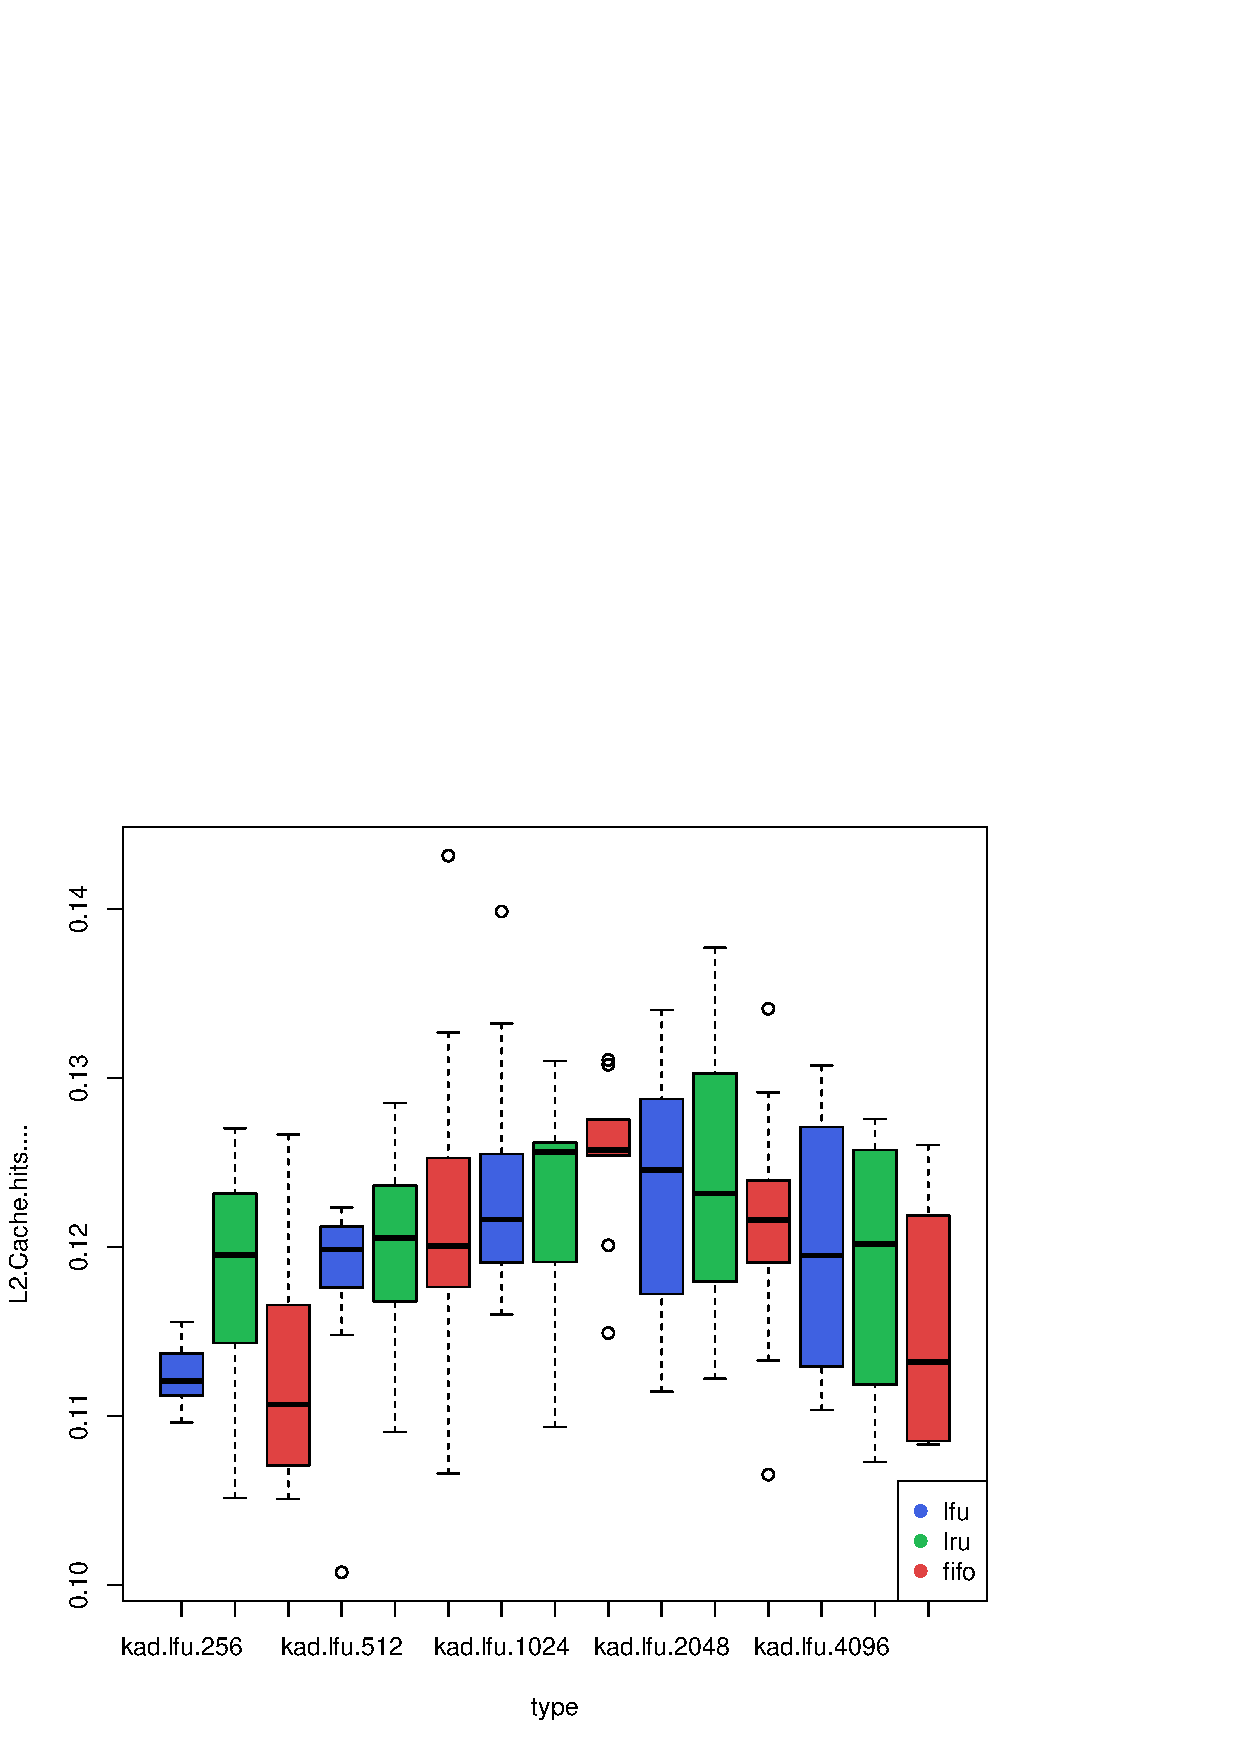
\includegraphics[width=0.85\linewidth]{img/cache.pdf}
\caption{
Przykład lokalnego serwera \keszujacego.
Zamiast wielokrotnie odwoływać się do docelowego serwera, który zawiera daną stronę
możemy zapamiętać ją na serwerze \keszujacym. Takie rozwiązanie niesie ze sobą zalety
zarówno dla administratorów serwera w~Chicago, jak i~użytkowników sieci w~Japonii:
mniej żądań skutkuje mniejszym obciążeniem serwera, a~,,lokalność'' serwera \keszujacego\s zmniejsza opóźnienia i~zwiększa szybkość transferu zasobu.
}
\label{fig_cache_server}
\end{figure}

Wprowadzenie \keszowania\s niesie ze sobą szereg zalet nie tylko dla administratorów serwerów zawierających zasoby. Serwery znajdujące się na granicy sieci lokalnej z~Internetem (jak na rysunku~\ref{fig_cache_server}) oferują użytkownikom tej sieci lepszy transfer i~mniejsze opóźnienia w~dostępie do popularnych zasobów.
Ponieważ łącze wychodzące z~sieci ma ograniczoną przepustowość, \kesz\s pozwala również na jego oszczędniejsze wykorzystanie, a~tym samym poprawę jakości dostępu do Internetu.

\subsection{Rozproszony i~hierarchiczny \kesz}\label{sect_dist_cache}
Rozwiązanie przedstawione w~rozdziale~\ref{sect_cache} pozwala na odciążenie serwera docelowego. Zastanówmy się jednak co będzie się działo w~przypadku zwiększania liczby użytkowników korzystających z~serwera \keszujacego. Duża liczba żądań może spowodować dokładnie taką samą sytuację jak w~przypadku serwera docelowego - \kesz\s zostanie zalany i~nie będzie w~stanie obsłużyć wszystkich zapytań.

W 1995 roku Malpani i~inni \cite{malpani1995making} zaproponowali metodę, w~której wiele serwerów \keszujacych\s współpracuje ze sobą w~celu zrównoważenia obciążenia. W~ich propozycji klient wysyła żądanie do losowego serwera należącego do systemu. W~przypadku, gdy serwer posiada określony zasób odsyła go w~odpowiedzi, w~przeciwnym razie rozsyła to żądanie do wszystkich innych serwerów. Jeżeli żaden z~\keszy\s nie zawiera zasobu, to żądanie jest przesyłane do serwera oryginalnego. Niestety wraz ze wzrostem liczby serwerów, należących do systemu liczba przesyłanych między nimi wiadomości bardzo szybko rośnie i~cały system staje się zawodny.

W ramach projektu Harvest \cite{bowman1994harvest} A. Chankhunthod i~inni \cite{chankhunthod1995hierarchical} stworzyli \kesz\s hierarchiczny. Rozwiązanie to pozwala łączyć kilka serwerów w~system, który można skalować w~zależności od liczby użytkowników, których ma obsługiwać. Grupy użytkowników łączą się z~serwerami, będącymi liśćmi w konstruowanej strukturze drzewa. Przychodzące żądania są obsługiwane najpierw przez serwery na najniższym poziomie, w~przypadku gdy te serwery nie mają danego zasobu w~\keszu\s decydują czy pobrać go z~serwera docelowego, czy odpytać serwery z~tego samego i~wyższego poziomu. Decyzja podejmowana jest na podstawie opóźnień do obu serwerów.

\begin{figure}[h]
\centering
\includegraphics[width=0.8\linewidth]{img/hierarchical.pdf}
\label{fig_cache_hierarchical}
\caption{Połączenie kilu serwerów \keszujacych\s w~system hierarchiczny. Każdy z~serwerów znajdujących się w~liściach obsługuje określoną liczbę użytkowników. Zapytania o~zasoby, które nie znajdują się w~\keszu\s wysyłane są do rodzica.}
\end{figure}

W praktyce, w~takim systemie serwery na wyższych poziomach muszą obsługiwać dużą liczbę żądań od dzieci przez co stają się wrażliwe na zalanie oraz składują duże ilości danych \cite{povey1997distributed}.

Kolejnym zaproponowanym udoskonaleniem jest \kesz\s rozproszony. Rozwiązanie zachowuje hierarchiczną strukturę w~formie drzewa, ale tym razem jedynie serwery w~liściach zajmują się \keszowaniem\s zasobów, a~pozostałe serwery stanowią indeks, w~którym zapamiętywana jest informacja czy zasób znajduje się w~systemie oraz jaki serwer go przechowuje.

Jak pokazały eksperymenty \cite{povey1997distributed} rozproszony \kesz\s oferuje zbliżoną wydajność do \keszu\s hierarchicznego rozwiązując dodatkowo problemy związane z~obsługą dużej liczby żądań przez serwery na wyższych poziomach.

\subsection{Dynamiczna restrukturyzacja}
Przedstawione w~rozdziałach~\ref{sect_cache} i~\ref{sect_dist_cache} metody \keszowania\s nie są przystosowane do działania w~warunkach, w~których obciążenie czy liczba użytkowników obsługiwanych przez system się zmienia. Wraz z~rosnącą liczbą żądań nie jest możliwe łatwe poprawienie wydajności przez dołożenie dodatkowych serwerów \keszujacych. Wprowadzenie zmian w~systemie wymaga zmian w~konfiguracji poszczególnych serwerów. Dodatkowo awarie pojedynczych węzłów mogą spowodować nieprawidłową pracę \keszu.

W celu ułatwienia dodawania i~usuwania serwerów do systemu możemy spróbować innego podejścia do problemu. Podstawowym zadaniem węzłów wewnętrznych w~systemie \keszu\s rozproszonego jest utrzymywanie indeksu przechowywanych zasobów i~lokalizacja serwera, który dany zasób obsługuje. Zatem jeżeli klient mógłby określić, który serwer \keszujacy\s jest odpowiedzialny za obsługę obiektu, wtedy cała infrastruktura związana z~indeksowaniem byłaby niepotrzebna.

Naiwnym rozwiązaniem stosującym takie podejście jest przypisanie zasobów do konkretnych serwerów. Przyjmijmy za identyfikator zasobu jego adres. Możemy teraz przypisać wszystkie zasoby w~obrębie jednej domeny do pewnego serwera. Na przykład dysponując 24 serwerami możemy przypisać wszystkie domeny zaczynające się na ,,a'' do serwera pierwszego, na ,,b'' do drugiego itd. Oczywiście pozwoli to na łatwe określenie, który serwer należy odpytać o~dany zasób, ale rozwiązanie to ma dwie poważne wady. Po pierwsze rozwiązanie nie jest skalowalne - niezdefiniowane jest jakie zasoby miałby obsługiwać dodatkowy serwer, a~po drugie obciążenie na serwerach jest nierównomierne.

Możemy jednak spróbować rozwiązać problem przydziału zasobów do serwerów nieco inaczej. Niech $n$ oznacza liczbę serwerów, a~$R$ adres pewnego zasobu, wtedy:
\begin{equation*}
S \equiv hash(R) \bmod n,
\end{equation*}
 gdzie $S$ oznacza indeks serwera odpowiedzialnego za zasób $R$, a~$hash$ jest funkcją haszującą. Dzięki właściwościom funkcji haszujących gwarantujemy, że zasoby każdy z~serwerów jest odpowiedzialny za równą część składowanych zasobów. Niestety dalej nie jest rozwiązany problem skalowalności. Dodanie ($n+1$)-go serwera powoduje, że wszystkie zasoby zostaną przypisane w~inne miejsca.
 
\subsubsection{\textit{Consistent Hashing}}
\label{sect_consistent_hashing}
Podczas dodawania nowego serwera do systemu oczekujemy, że przejmie on od pozostałych równą część zasobów, aktualnie znajdujących się w~\keszu. Dodatkowo nie chcemy, aby wartości w~\keszu\s były przesuwane pomiędzy ,,starymi'' serwerami. Taką własność gwarantuje mechanizm \textit{Consistent Hashing}, opracowany przez Kargera i~Lehmana \cite{karger1997consistent}.

Załóżmy, że dysponujemy funkcją haszującą w~odcinek $[0, 1]$, za pomocą której każdemu zasobowi i~serwerowi przyporządkowujemy punkt na tym odcinku. Dodatkowo, traktujemy odcinek jako okrąg o~obwodzie równym 1. W~podanym przez Kargera i~Lehmana schemacie dany zasób jest obsługiwany przez najbliższy serwer idąc zgodnie z~ruchem wskazówek zegara. Rysunek~\ref{fig_consistent_hashing} przedstawia przykładowe mapowanie zasobów i~ich przyporządkowanie do poszczególnych serwerów. W~drugiej części rysunku przedstawiona została zmiana przyporządkowania wynikająca z~dodania nowego serwera $D$.

\begin{figure}[ht]
\centering
\begin{minipage}[b]{0.445\linewidth}
\centering
\includegraphics[width=0.95\textwidth]{img/consistent.pdf}
\end{minipage}
\begin{minipage}[b]{0.47\linewidth}
\centering
\includegraphics[width=0.95\textwidth]{img/consistent_2.pdf}
\end{minipage}
\caption{Idea \textit{Consistent Hashing}. Zasoby, reprezentowane przez zielone punkty, oraz serwery \keszujace\s (kwadraty) mapowane są na punkty na okręgu o~jednostkowym obwodzie. W~praktyce do reprezentowania punktów na okręgu najczęściej wykorzystywane są klucze binarne o~ustalonej długości $m$. Każdy serwer jest odpowiedzialny za obsługę zasobów znajdujących się pomiędzy jego punktem i~punktem jego poprzednika. Dodanie nowego serwera $D$ powoduje wyłącznie zmianę przydziału zasobu $4$.}
\label{fig_consistent_hashing}
\end{figure}

W praktyce, przesłanie informacji dotyczących zmian serwerów do wszystkich klientów byłoby bardzo kosztowne, ale sytuacja, w~której klienci mają różne ,,widoki'' (wiedzą tylko o~pewnym podzbiorze serwerów) systemu nie stanowi problemu po wprowadzeniu prostej modyfikacji. Zauważmy, że może dojść do sytuacji, w~której jeden z~serwerów, z~powodu niepełnej wiedzy klientów, będzie obsługiwał więcej żądań od pozostałych. W~celu rozwiązania nierównego obciążenia autorzy zaproponowali stworzenie wirtualnych kopii serwerów, tzn. każdy z~nich zmapowany jest nie do jednego, lecz kilku punktów na okręgu. Dzięki temu z dużym prawdopodobieństwem zasoby będą równomierne przyporządkowane do serwerów \cite{karger1999web}.

Pomimo, że pierwotną motywacją powstania \textit{Consistent Hashing} był problem \keszowania\s zasobów internetowych, schemat znalazł zastosowanie w~innych obszarach. W~szczególności, leży on u~podstaw rozproszonych tablic haszujących, które omówione są w~rozdziale~\ref{sect_dht}.

\section{Rozproszone tablice haszujące (DHT)}
\label{sect_dht}
Rozproszone tablice haszujące (ang. \textit{Distributed Hash Tables}, DHT) to systemy pozwalające na przechowywanie par \textit{(klucz, wartość)}, podobnie jak zwykłe tablice haszujące, w~dynamicznej sieci zbudowanej z~uczestniczących węzłów (\textit{peer-to-peer}). Odpowiedzialność za przetrzymywanie mapowania kluczy do wartości jest podzielona pomiędzy węzły, w~taki sposób aby zmiany w~liczbie uczestników nie powodowały reorganizacji całości systemu, ale tylko jego drobnej części. Dodatkowo rozproszone tablice haszujące oferują efektywne wyszukiwanie kluczy w~systemie.

Początkowe badania nad DHT były motywowane istniejącymi systemami peer-to-peer, oferującymi głównie możliwość dzielenia się plikami, np. \textit{Napster}, \textit{Gnutella} i~\textit{Freenet}. Sieci te na różne sposoby realizowały wyszukiwanie zasobów, ale każdy z~nich miał swoje wady. \textit{Napster} korzystał z~centralnego katalogu, do którego każdy serwer wysyłał swoją listę plików i~który zarządzał wyszukiwaniem plików. W~\textit{Gnutelli} w~celu odnalezienia zasobu, zapytanie wysyłane było do każdego węzła w~sieci w~określonym promieniu, co skutkowało mniejszą szybkością i~mnóstwem przesyłanych wiadomości oraz podobnie jak w~przypadku sieci \textit{Freenet}, w~której znajdowanie klucza odbywało się za pomocą heurystycznej metody, brak gwarancji odnalezienia klucza.

Idea rozproszonych tablic haszujących ma na celu rozwiązanie wszystkich przedstawionych problemów:
\begin{itemize}
  \item w~pełni rozproszony, skalowalny system; brak centralnego zarządzania,
  \item odporność na awarie węzłów,
  \item deterministyczny algorytm routingu, z~dowiedzioną poprawnością, pozwalający na efektywne wyszukiwanie. 
\end{itemize} 

Jedną z~pierwszych sieci DHT, bazujących na schemacie \textit{Consistent Hashing} jest \textit{Chord}, opisany w~rozdziale~\ref{sect_dht_chord}.

\subsection{Chord}
\label{sect_dht_chord}
Sieć \textit{Chord} opracowana przez Stoicę, Morrisa, Kargera, Kaashoeka i~Balakrishnana  \cite{stoica2001chord} to jedna z~czterech pierwszych powstałych rozproszonych tablic haszujących\footnote{Pozostałe to CAN\cite{ratnasamy2001scalable}, Tapestry \cite{zhao2001tapestry} i~Pastry\cite{rowstron2001pastry}.}. Zapewnia szybki i~odporny na błędy protokół routingu, znajdujący węzeł odpowiedzialny za dany klucz w~czasie logarytmicznym w~stosunku do liczby węzłów w~sieci.

U podstaw \textit{Chorda} leży mechanizm \textit{Constistent Hashing} opisany w~rozdziale~\ref{sect_consistent_hashing}. W~przypadku \textit{Constistent Hashing}, aby zlokalizować węzeł odpowiedzialny za dany klucz wymagana była znajomość wszystkich węzłów w~sieci. Takie rozwiązanie pozwala na szybkie odnalezienie węzła, ale nie daje możliwości skalowania na dowolną liczbę węzłów. W~uproszczonej wersji \textit{Chorda}, w~celu zapewnienia efektywnego skalowania, autorzy wymagają wyłącznie znajomości przez węzeł swojego następnika. Dzięki temu, niezależnie od wielkości sieci każdy z~węzłów przechowuje informacje tylko o~jednym sąsiedzie, ale czas odnalezienia dowolnego klucza jest liniowy w~stosunku do liczby węzłów (wiadomości są przesyłane po pierścieniu aż dotrą do docelowego serwera).

\begin{figure}[h!]
\centering
\includegraphics[width=0.5\linewidth]{img/chord.pdf}
\caption{Kontakty (\textit{fingers}) węzła $A$ w~sieci Chord. Dla ustalonej długości klucza $m$, węzeł $n$ przechowuje kontakty: $successor(n + 2^{i-1})$ dla każdego $i = 1, 2, \dots,  m$; gdzie $successor(k)$ oznacza serwer odpowiedzialny za klucz $k$.}
\label{fig_chord_fingers_1}
\end{figure}

Bardziej efektywna wersja routingu zakłada, że każdy z~węzłów utrzymuje tabelę z~kontaktami w~określonych odległościach od niego samego. Kolejne kontakty są wykładniczo coraz bardziej odległe tak, jak przedstawione to zostało na rysunku~\ref{fig_chord_fingers_1}. Takie podejście pozwala na odnalezienie węzła odpowiedzialnego za zadany klucz w~czasie $O (\log n)$. Aby łatwiej zauważyć tę własność, możemy przedstawić kontakty w~formie drzewa (rysunek~\ref{fig_chord_fingers_2}). Każdy krok w~routingu \textit{Chorda} skraca wtedy pozostały dystans co najmniej o~połowę.


\begin{figure}[h!]
\centering
\includegraphics[width=0.9\linewidth]{img/chord_2.pdf}
\caption{Kontakty węzła $A$ w~sieci Chord w~postaci drzewa. Węzeł ma możliwość kontaktowania się z~pojedynczymi węzłami w~kolejnych poddrzewach, o~co raz większej wysokości.}
\label{fig_chord_fingers_2}
\end{figure}

Podczas dołączania do sieci węzeł $n$ musi znać adres co najmniej jednego węzła, który należy już do sieci, nazwijmy go $n'$. Procedura dołączania polega na poproszeniu $n'$ o~znalezienie następnika dla $n$. W~kolejnym kroku $n$ buduje tablicę kontaktów wysyłając zapytania o~$successor(n + 2^{i-1})$ dla każdego kolejnego $i$. Po zakończeniu tego procesu $n$ posiada pełną listę kontaktów, ale tylko jego następnik wie o~jego istnieniu.

Pozostałe węzły mają możliwość uwzględnienia nowych podczas cyklicznego wykonywania procedury stabilizacyjnej, odpowiadającej za uaktualnienie (poprawienie) informacji o~poprzedniku i~następniku dla każdego węzła. Dodatkowo również cyklicznie wywoływana jest procedura, która odpowiada za uaktualnianie tabel kontaktów.

\textit{Chord} stanowi implementację mechanizmu \textit{Constistent Hashing} w sieci peer-to-peer. Dzięki dobrym właściowościom (logarytmiczny routing) oraz prostocie działania sieć ta jest bardzo często wykorzystywana do opisu bardziej zaawansowanych algorytmów, takich jak równoważenie obciążenia \cite{rao2003load}, usprawnienia routingu \cite{manku2004know} i tym podobnym. Jednakże w praktycznych zastosowaniach, kiedy część z węzłów może nie odpowiadać (lub może odpowiadać wolno), algorytm routing w \textit{Chordzie} podczas jednego kroku kontaktuje się tylko z jednym węzłem i musi czekać na jego odpowiedź, co może powodować znaczne opóźnienia. 


\subsection{Kademlia}
W 2002 roku Maymounkov i~Mazieres opracowali nową sieć P2P, która wykorzystywała zalety pierwszych sieci oraz uwzględniała nie tylko aspekty teoretyczne, ale również wykorzystanie sieci w~praktyce.

\textit{Kademlia} \cite{maymounkov2002kademlia}, podobnie jak pierwsze powstałe sieci peer-to-peer, pozwala na odnalezienie zasobu w~czasie logarytmicznym względem liczby węzłów w~sieci. Zaletą \textit{Kademli} jest fakt, że każdy pakiet wymieniany pomiędzy węzłami niesie ze sobą dodatkowe, użyteczne informacje o~pozostałych węzłach, dzięki czemu nie jest konieczne wysyłanie dodatkowych komunikatów, niezbędnych do działania systemu. Wykorzystanie tej własności umożliwia użycie metryki odległości opartej na funkcji XOR, co więcej sieć pozwala na równoległe odpytywanie wielu węzłów w~celu zmniejszenia opóźnień użytkownika. Szczegóły działania routingu \textit{Kademli} zostały opisane w~rozdziale~\ref{kad_routing}.

W celu identyfikacji zasobów i~węzłów w~sieci \textit{Kademlia} używane są 160-bitowe klucze (np. hash SHA-1 identyfikatora). Zasoby są składowane w~węzłach, których klucz jest blisko identyfikatora zasobu. W~celu określenia "bliskości" elementów wykorzystywana jest metryka XOR, tzn. im więcej początkowych bitów dwóch kluczy jest zgodnych tym bliżej siebie się znajdują. Dzięki temu, że funkcja XOR jest symetryczna każde zapytanie, które dociera do danego węzła, może nieść ze sobą informacje o~nowym kontakcie, którym jest nadawca komunikatu.

Każdy węzeł utrzymuje swoją tablicę kontaktów wykorzystywaną podczas wyszukiwania zasobów. Tablica dla węzła o~identyfikatorze $X$ składa się z~$k$-pojemników (ang. \textit{$k$-buckets}), które dla każdego $i \in [0, 160)$ przechowują adresy (maksymalnie) $k$ węzłów, które znajdują się w~odległości od $2^i$ do $2^{i+1}$ od danego węzła. Zatem klucze w~$i$-tym pojemniku mają z~$X$ wspólny prefiks długości $160-(i+1)$, ale różnią się na bicie $160-i$. Parametr $k$ jest stały i~ustalony dla danej sieci (autorzy \textit{Kademli} proponują wartość $k=20$). Na rysunku~\ref{fig_kademlia} przedstawiona została przykładowa sieć dla kluczy długości $3$ oraz kontakty węzła o~kluczu $000$. 

Bazując na zapisach logów zebranych przez Saroiu i~innych \cite{saroiu2001measurement} z~działającej sieci \textit{Gnutella}, zaobserwowano, że prawdopodobieństwo, że węzeł który znajduje się w~sieci od $x$ minut będzie się w~niej znajdował również w~czasie $x+60$ rośnie wraz ze wzrostem $x$. Własność ta została wykorzystana w~\textit{Kademli} w~celu ustalenia kolejności w~$k$-pojemnikach. Węzły są uszeregowane według malejącego czasu ostatniej widoczności\footnote{Czas ten jest uaktualniany w~momencie otrzymywania zapytań lub odpowiedzi na zapytania od danego węzła.}. W~momencie kiedy do danej listy ma trafić kolejny węzeł do ostatniego węzła na liście wysyłany jest komunikat w~celu sprawdzenia czy jest wciąż aktywny. W~przypadku braku odpowiedzi węzeł jest usuwany z~listy, a~nowy węzeł wstawiany jest na początek. W~przeciwnym razie węzeł jest przesuwany na początek listy, a~nowy kontakt jest ignorowany. Dzięki takiemu podejściu sieć dodatkowo staje się częściowo odporna na ataki, w~których adwersarz wprowadza wiele nowych węzłów, które mają na celu "wypchnięcie" prawdziwych węzłów z~tabel kontaktów.

\begin{figure}[h]
\centering
\includegraphics[width=0.9\linewidth]{img/kademlia.pdf}
\caption{Tablica kontaktów węzła $000$ w~przykładowej sieci \textit{Kademli}. Szare elipsy oznaczają kolejne $k$-pojemniki. Rysunek ten bardzo przypomina rysunek~\ref{fig_chord_fingers_2}. W~przypadku \textit{Chorda} węzeł znał co najwyżej jeden węzeł z~każdego poddrzewa. Dzięki zastosowaniu metryki XOR w~\textit{Kademli} węzły bez dodatkowych komunikatów mogą dowiedzieć się o~pozostałych węzłach, które należą do danego przedziału. Informacja ta wykorzystywana jest w~celu przyspieszenia routingu w~praktycznych zastosowaniach.}
\label{fig_kademlia}
\end{figure}

\subsubsection{Routing}
\label{kad_routing}
Protokół \textit{Kademli} oparty jest o~cztery procedury: \f{STORE}, \f{PING}, \f{FIND\_NODE} oraz \f{FIND\_VALUE}. Pierwsza procedura wysyła prośbę o~zapamiętanie pary (klucz, wartość). \f{PING} używany jest do ustalenia czy dany węzeł powinien zostać usunięty z~pewnego $k$-pojemnika lub czy dalej jest aktywny. Dwie kolejne procedury stanowią najważniejszą część sieci. Obie używają tego samego algorytmu routingu w~celu odnalezienia węzła lub wartości, która reprezentowana jest przez zadany klucz.

W celu odnalezienia węzła o~kluczu $X$ przez węzeł $S$ na podstawie tablicy kontaktów określanych jest $k$ najbliższych do klucza $X$ węzłów sieci. W~kolejnym kroku $S$ przesyła zapytanie o~$k$ najbliższych węzłów do węzłów wybranych w~poprzednim kroku. Dzięki zastosowanej metryce XOR i~jej własnościom możliwe jest wysyłanie równoczesnych zapytań do kilku węzłów. Liczbę równoległych żądań określa parametr $\alpha$, dla którego Maymounkov i~Mazieres proponują wartość 3. Dzięki odpytywaniu wielu węzłów w~tym samym czasie możemy uzyskać krótszy czas dostępu do zasobów, w~przypadku gdy część węzłów nie odpowiada na komunikaty węzła $S$. Procedura \f{FIND\_VALUE} obsługiwana jest dokładnie w~ten sam sposób, dopóki jeden z~węzłów nie posiada wartości odpowiadającej danemu kluczowi. Wtedy węzeł zamiast zwracać $k$ najbliższych węzłów zwraca po prostu wartość, znajdującą się pod podanym kluczem.

\textit{Kademlia}, dzięki zastosowaniu metryki XOR pozwala na znaczące uproszczenie zarówno analizy poprawności i złożoności routingu, jak i implementacji. Dodatkowo możliwość zastosowania równoległych, asynchronicznych zapytań do wielu węzłów naraz niesie ze sobą duże zalety praktyczne. Podejście to pozwala na zmniejszenie opóźnień spowodowanych nieodpowiadającymi serwerami. Ponieważ, w przeciwieństwie do \textit{Chorda}, dwa różne zapytania o te same klucze od pewnego miejsca będą zbiegały wzdłuż tej samej ścieżki możliwe jest powielanie popularnego zasobu na węzłach leżących na tej ścieżce. Dzięki temu klienci, którzy obsługują często wyszukiwane zasoby nie zostaną zablokowani z powodu nadmiernej ilości zapytań, ponieważ część odpowiedzi będzie udzielanych już na wcześniejszym etapi routingu.

\section{Rozproszony \kesz\s z~użyciem DHT}
\label{sect_cache_dht}
Obecne zastosowania DHT skupiają się głównie na systemach wymiany plików takich jak Kad czy BitTorrent. W~systemach tych DHT są używane w~celu odnalezienia komputerów, które przechowują dany plik. W~tej pracy proponujemy użycie DHT w~celu \keszowania\s zasobów internetowych. Jak opisane zostało w~rozdziale~\ref{sect_consistent_hashing} \keszowanie\s zasobów leżało u~podstaw powstania mechanizmu \textit{Consistent Hashing}, który z~kolei zapoczątkował rozwój DHT.

\subsection{Motywacja}
Pod koniec lat dziewięćdziesiątych, kiedy opracowane zostało \textit{Constistent Hashing} z~internetu korzystało 7\% światowej populacji (31\% w~krajach rozwiniętych)\cite{wiki:GlobalStats}. Problemy, które stały wówczas przed twórcami mechanizmu rozpatrywane były głównie z~punktu widzenia serwerów, których zalanie nadmierną liczbą zapytań powodowało czasowe problemy z~dostępem do zasobów. Rozwiązania miały na celu stworzenie infrastruktury, która pozwalałaby na odciążenie serwerów i~w efekcie zwiększenie dostępności danych.

Obecnie, około 13 lat później, Internet i~jego użycie zmieniło się diametralnie. Liczba użytkowników Internetu podwoiła się w~krajach rozwiniętych (do poziomu 77\%) oraz wzrosła ponad pięciokrotnie (do 39\%) biorąc pod uwagę całą populację\cite{wiki:GlobalStats}. Wraz z~rozwojem sieci rozwijała się też technologia. Obecne serwery mogą sprostać o~wiele większemu obciążeniu. Pojawiły się również dodatkowe rozwiązania pozwalające na łatwiejsze skalowanie dużych stron internetowych takie jak CDN (\textit{Content Delivery Network}) oraz \textit{Cloud-based hosting}.

Jakkolwiek oryginalna motywacja \keszowania\s straciła obecnie na znaczeniu, to jednak współczesny Internet stawia szereg nowych problemów, którym musimy sprostać. Wraz ze wzrostem popularności serwisów, które zajmują się agregowaniem treści (jak \textit{reddit\footnote{\url{http://reddit.com}}} oraz \textit{Wykop\footnote{\url{http://wykop.pl}}}) coraz większym problemem staje się tzw. \textit{Slashdot Effect}. Efekt obserwowany jest kiedy strona ciesząca się pierwotnie niewielkim lub umiarkowanym zainteresowaniem trafia do agregatora, dzięki któremu w~krótkim czasie zyskuje olbrzymi wzrost liczby wizyt. W~rezultacie serwer, który nigdy nie był przygotowany do obsługi tak wielu zapytań zostaje zalany i~staje się niedostępny. Na wykresie~\ref{fig_slashdot} przedstawiony został wzrost ilości przesyłanych danych spowodowany przez \textit{Slashdot Effect}.

\begin{figure}[h!]
\centering
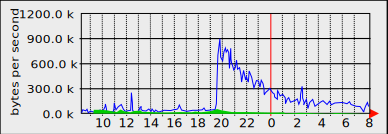
\includegraphics[width=0.9\linewidth]{img/SlashdotEffectGraph.pdf}
\figsource{https://en.wikipedia.org/wiki/File:SlashdotEffectGraph.svg}
\caption{Wykres ilości danych przesyłanych przez serwer. Około godziny 20:00 można zaobserwować olbrzymie zwiększenie ruchu spowodowane efektem \textit{Slashdot}}
\label{fig_slashdot}
\end{figure}

W dzisiejszych czasach problemem jest nie tylko chwilowa zwiększona ilość ruchu, spowodowana efektem \textit{Slashdot}, ale przede wszystkim objętość przesyłanych danych. Porównując dane z~roku 2000 oraz 2007 możemy zaobserwować ponad trzykrotny wzrost rozmiaru danych przesyłanych z~internetu\cite{sadre2008changes}. Na rysunku~\ref{fig_mean_webpage}, przedstawiającym wykres średniego rozmiaru strony\footnote{Strony rozumianej jako dokument HTML, obrazki, skrypty itd.}, ponownie widoczna jest zdecydowana tendencja wzrostowa. Na podstawie wykresu możemy wyciągnąć wniosek, że średni rozmiar strony podwaja się co około trzy lata. Dodatkowo, obecna sieć pełna jest obiektów o~dużym rozmiarze (filmy, multimedia), które rzadko są \keszowane\s z~powodu ograniczonych zasobów na scentralizowanych serwerach \keszujacych\s\cite{sadre2008changes}.

\begin{figure}[h!]
\centering
\includegraphics[width=0.7\linewidth]{img/mean_webpage_size.eps}
\captionsetup{font={scriptsize, it}}
\caption*{Opracowane na podstawie: \url{http://httparchive.org} oraz \url{http://www.pantos.org/atw/35654.html}.}
\captionsetup{font={normalsize}}
\caption{Wykres średniego rozmiaru strony w~poszczególnych latach. W~ciągu ostatnich 3 lat średni rozmiar strony podwoił się.}
\label{fig_mean_webpage}
\end{figure}

System \keszujacy\s oparty o~sieć peer-to-peer, proponowany w~tej pracy stara się adresować przedstawione problemy. W~celu zwiększenia pojemności i~umożliwienia \keszowania\s multimediów system wykorzystuje rozproszone zasoby uczestników sieci w~celu odciążenia serwerów i~zmniejszenia opóźnień użytkowników. Szczegóły dotyczące architektury proponowanego rozwiązania opisane zostały w~rozdziale~\ref{sect_architecture}.

\subsection{Poprzednie prace}
\label{sect_previous_work}
Problem \keszowania\s zasobów opisywany był w~literaturze wielokrotnie. Jako przykłady warto ponownie przytoczyć prace \cite{malpani1995making, chankhunthod1995hierarchical, povey1997distributed} omawiane już w~rozdziale~\ref{sect_dist_cache}. Niezwykle ważne w~historii \keszowania\s są prace Kargera i~innych \cite{karger1997consistent, karger1999web} wprowadzające mechanizm \textit{Consistent Hashing}.

Idea użycia potencjalnie nieograniczonych zasobów sieci peer-to-peer w~celu \keszowania\s zasobów internetowych pojawia się w~pracy \cite{iyer2002squirrel, clevenot2004simple}, przedstawiającej system \textit{Squirrel}. \textit{Squirrel} oparty jest o~sieć Pastry\cite{rowstron2001pastry}. 
Na podobnym pomyśle bazuje \textit{Tuxedo} \cite{shi2003tuxedo}, który dodatkowo stara się \keszowac\s również zasoby, które są spersonalizowane, jednak wymaga scentralizowanej konfiguracji i~nie jest przystosowany do użycia przez użytkowników końcowych. 
Kolejną siecią opartą na unikalnej implementacji DHT jest \textit{Kache}\cite{linga2004kache}, używający opracowanej na własne potrzeby sieci \textit{Kelips}.
Ciekawy pomysł zastosowania sieci peer-to-peer w~celu przyspieszania strumieniowania multimediów został opisany w~\cite{guo2006design}.

Pomimo podobnej tematyki przytoczonych prac żadna z~nich nie wykorzystuje sieci \textit{Kademlia}, oferującej pewne zalety istotne w~zastosowaniach praktycznych, w~szczególności równoległe zapytania w~trakcie routingu.

\subsection{Architektura}
\label{sect_architecture}
Opracowana aplikacja składa się z~dwóch głównych części: serwera proxy oraz klienta sieci peer-to-peer. Oba komponenty połączone są ze sobą przez zarządcę \keszu.

\begin{figure}[h!]
\centering
\includegraphics[width=0.9\linewidth]{img/architecture.pdf}
\caption{Przekrój architektury systemu. Składowa \textit{Two-level cache} odpowiada za zarządzanie \keszem. W~pierwszej kolejności odpytywany jest lokalny \kesz\s w~pamięci, w~przypadku gdy poszukiwana wartość nie została znaleziona zapytanie wysyłane jest do sieci P2P. Jeżeli zasób nie zostanie znaleziony w~żadnym z~dostępnych \keszy\s serwer proxy wyśle żądanie do serwera oryginalnego, a~następnie umieści odpowiedź serwera w~obu typach \keszu.}
\label{fig_architecture}
\end{figure}

Serwer proxy odpowiada za obsługę żądań przychodzących od przeglądarki. Następnie odpytywany jest zarządca \keszu. W~zależności od wybranego typu \keszowania\s sprawdzany jest \kesz\s w~pamięci lub zapytanie wysyłane jest do \keszu\s rozproszonego w~sieci peer-to-peer. Po otrzymaniu odpowiedzi z~sieci P2P jeżeli zasób został znaleziony to jego wartość zwracana jest do klienta, a~w przeciwnym przypadku serwer proxy wysyła zapytanie do serwera oryginalnego. Po otrzymaniu odpowiedzi zostanie ona umieszczona w~\keszu.

Dzięki modularnej budowie aplikacji każdy z~komponentów może zostać łatwo podmieniony. Dostępne są trzy implementacje polityk usuwania elementów z~\keszu\s w~przypadku przepełnienia: \textit{First In First Out(FIFO)}, \textit{Least Recently Used (LRU)} oraz \textit{Least Frequently Used (LFU)}. Pierwszy z~algorytmów, jeżeli brakuje miejsca na nowy element, usuwa z~\keszu\s element, który dodany został do niego jako pierwszy. \textit{LRU} z~kolei usuwa ten, który był używany najdawniej. \textit{LFU} usuwa element, który używany był najrzadziej (w przypadku takiej samej częstotliwości użycia usuwany jest element zgodnie z~polityką \textit{FIFO}). Opisane polityki mogą zostać użyte jako algorytm zarządzania \keszem\s w~pamięci. 

Aplikacja pozwala na wybranie jako implementację DHT jednej z~dwóch z~sieci: Chord lub Kademlia. Obie sieci w~celu składowania zasobów mogą użyć dowolnego z~opisanych algorytmów \keszowania.

W przeciwieństwie do większości tego typu systemów opisywanych w~literaturze, w~przypadku dołączania i~odchodzenia węzłów do sieci nie są podejmowane żadne akcje mające na celu albo wypełnienie lokalnego \keszu\s nowo dołączonego klienta, albo przesłanie swoich zasobów pozostałym węzłom w~przypadku odchodzenia. Pomimo, że takie podejście może zwiększać liczbę zapytań, które będą musiały zostać obsłużone z~serwerów oryginalnych, to pozwala na uniknięcie efektu zwanego \textit{churn}. \textit{Churn} to nadmierna komunikacja wewnątrz sieci, która spowodowana jest częstym i~szybkim dochodzeniem i~odchodzeniem węzłów.  

\section{Testy}
\label{sect_tests}
Do analizy prezentowanej aplikacji stworzony został symulator pozwalający na przetestowanie działania różnych możliwych konfiguracji. Symulator pozwala na wczytanie danych dotyczących węzłów w~sieci i~zapytań, które wysyłają w~określonym czasie. 

W celu jak najlepszego oddania realnych warunków pracy systemu w~trakcie symulacji dla każdego klienta uruchamiany jest osobny proces systemowy z~działającym programem. Następnie do tego procesu wysyłane są adresy i~czasy, w~których klient ma wysłać zapytania na dany adres. Dzięki takiemu podejściu kompleksowo testowana jest niemal cała architektura przedstawiona na rysunku~\ref{fig_architecture}. Jedynym komponentem, który nie bierze udziału w~symulacji jest serwer proxy, ponieważ zapytania są tworzone bezpośrednio przez procesy klientów.

Do uruchomienia symulacji wymagany jest plik zawierający listę wszystkich klientów, oraz osobny plik dla każdego klienta zawierający zapytania, które ma wykonać w~trakcie symulacji. Symulator tworzy procesy dla wszystkich klientów podczas startu, każdy z~nich dołącza też do sieci P2P na samym początku. Jednak po wysłaniu wszystkich swoich zapytań klient opuszcza sieć bez informowania żadnego z~węzłów.

\subsection{Dane testowe}
Jako dane wejściowe do symulatora użyte zostały realne dane pochodzące z~działających centralnych serwerów \keszujacych. Niestety znalezienie aktualnych danych do testów jest obecnie niezwykle trudne ze względu na kwestie bezpieczeństwa i~anonimowości użytkowników takich serwerów. Niedostępne są też dane, które używane są w~podobnych pracach (wspomnianych w~rozdziale~\ref{sect_previous_work}) co powoduje, że porównanie systemu z~innymi staje się trudne. 

Dane, na których przeprowadzane były testy pochodzą z~2007 roku i~są danymi zebranymi przez serwer \keszujacy\s IRCache\footnote{\url{ftp://ftp.ircache.net/Traces/DITL-2007-01-09/}}. Do testów użyte zostały trzy zbiory danych \f{sj.sanitized20070110}, \f{sv.sanitized20070110} oraz \f{uc.sanitized20070109}.
Wszystkie użyte pliki zawierają zapytania wykonywane przez klientów w~ciągu jednej doby. Liczba wysyłanych zapytań oraz liczba klientów dla poszczególnych plików przedstawiona została w~tabeli~\ref{tab_testdata}. W~tabeli~\ref{tab_testdata2} przedstawiona zostały statystyki dotyczące liczby wysyłanych zapytań przez pojedynczego klienta w~przedstawionych zbiorach danych. Wartości w kolejnych kolumnach oznaczają odpowiednio minimalną liczbę zapytań wykonaną przez pewnego klienta, medianę i średnią z liczby zapytań wszystkich klientów oraz maksymalną liczbę zapytań przypadającą na klienta w tym zbiorze danych.

\begin{table}[h!]
\centering
\begin{tabular}{r c c c}
Plik z~danymi & Liczba klientów & Łączna liczba zapytań & Liczba zapytań \f{GET}\\
\hline
\f{sj.sanitized} & 114 & $348~189$ & $346~405$\\
\f{sv.sanitized} & 91 & $447~696$ & $447~621$\\
\f{uc.sanitized} & 160 & $544~370$ & $527~355$\\
\end{tabular}
\caption{Szczegóły dotyczące użytych danych testowych.}
\label{tab_testdata}
\end{table}

\begin{table}[h!]
\centering
\begin{tabular}{r c c c c c}
 & \multicolumn{5}{c}{Liczba zapytań na klienta} \\
Plik z~danymi & 1. kwartyl & Mediana & Średnia & 3. kwartyl & Max \\
\hline
\f{sj.sanitized} & 17 & 150 & 2 273 & 1414 & 45 910  \\
\f{sv.sanitized} & 11 & 120 & 2 976 & 703 & 167 000 \\
\f{uc.sanitized} & 24 & 199 & 3 230 & 1766 & 87 390  \\
\end{tabular}
\caption{Szczegóły dotyczące liczby zapytań przypadających na pojedynczego klienta.}
\label{tab_testdata2}
\end{table}

Na potrzeby testów z~danych zostały wycięte wyłącznie zapytania typu \f{GET}, a~czas został przeskalowany o~czynnik \nicefrac{1}{18}, tak aby pojedyncza symulacja trwała około $1.5$ godziny.

\subsection{\Keszowanie\s w~pamięci}
\label{sect_tests_mem}
Pierwszym testowanym podczas symulacji komponentem jest lokalny \kesz. \Keszowanie\s takie utrzymywane jest w~pamięci w~celu szybkiego dostarczenia danych, które były już pobierane wcześniej.

Przeprowadzone testy uwzględniały różne wielkości \keszu\s oraz różne algorytmy decydujące o~tym, który element należy wyrzucić kiedy \kesz jest już pełny, a~powinien do niego trafić nowy wpis.

W trakcie testów \keszowania\s w~pamięci całkowicie wyłączony został komponent odpowiedzialny za \keszowanie\s w~sieci P2P, zatem dla każdego z~węzłów dane \keszowane\s były niezależnie.

Przetestowane zostały trzy algorytmy opisane w~rozdziale~\ref{sect_architecture} o~wielkościach: 1024, 2048, 4096, 8192 oraz 16384. 
Wyniki testów dla poszczególnych zbiorów danych znajdują się na rysunku \ref{fig_tests_mem_all}. Uśrednione wyniki dla wszystkich zbiorów danych testowych przedstawione zostały na rysunku~\ref{fig_tests_mem_1}.

\begin{figure}[h!]
\centering
\begin{minipage}{0.48\linewidth}
\centering
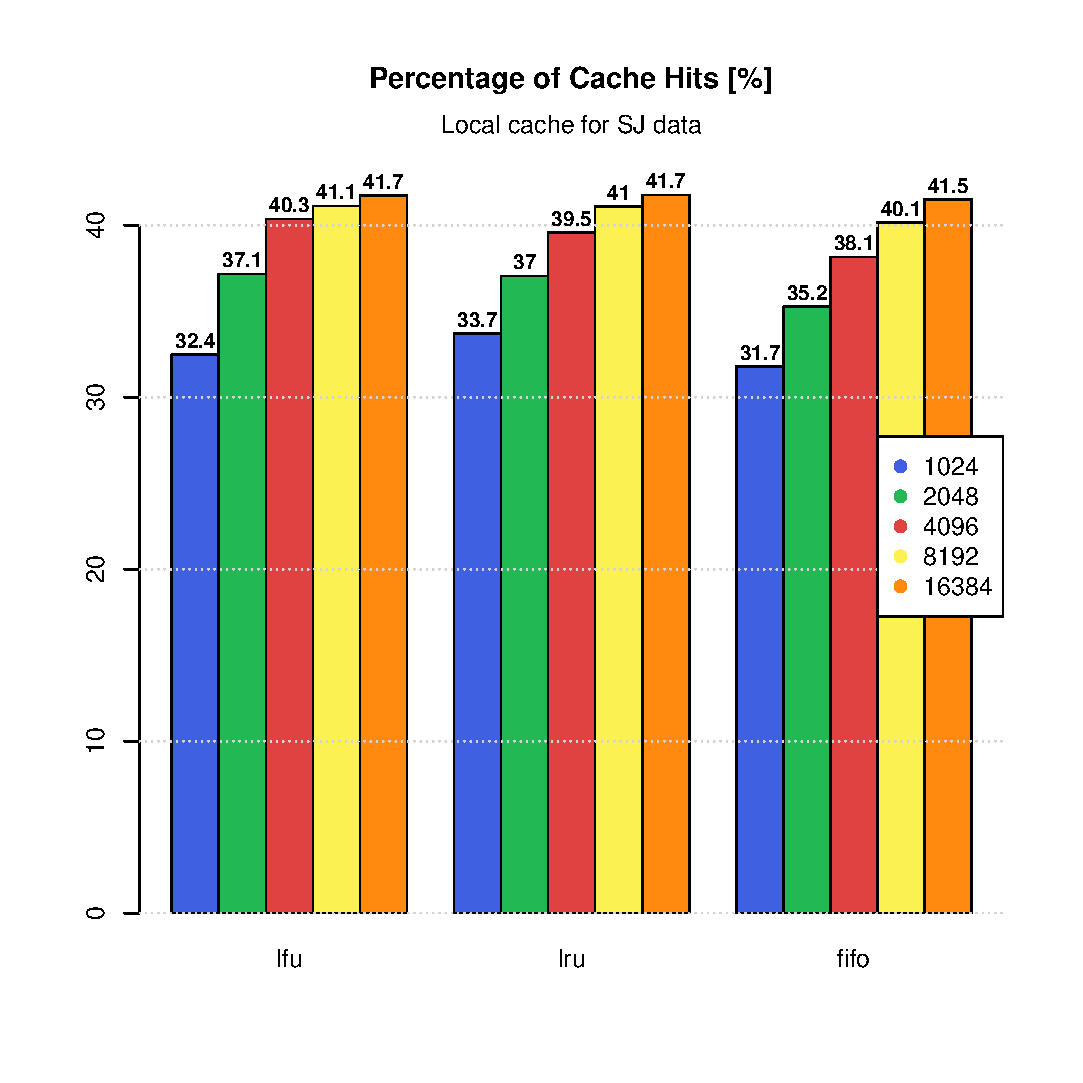
\includegraphics[width=0.9\linewidth]{img/tests/nop2p_sj_1.eps}
\end{minipage}
\begin{minipage}{0.48\linewidth}
\centering
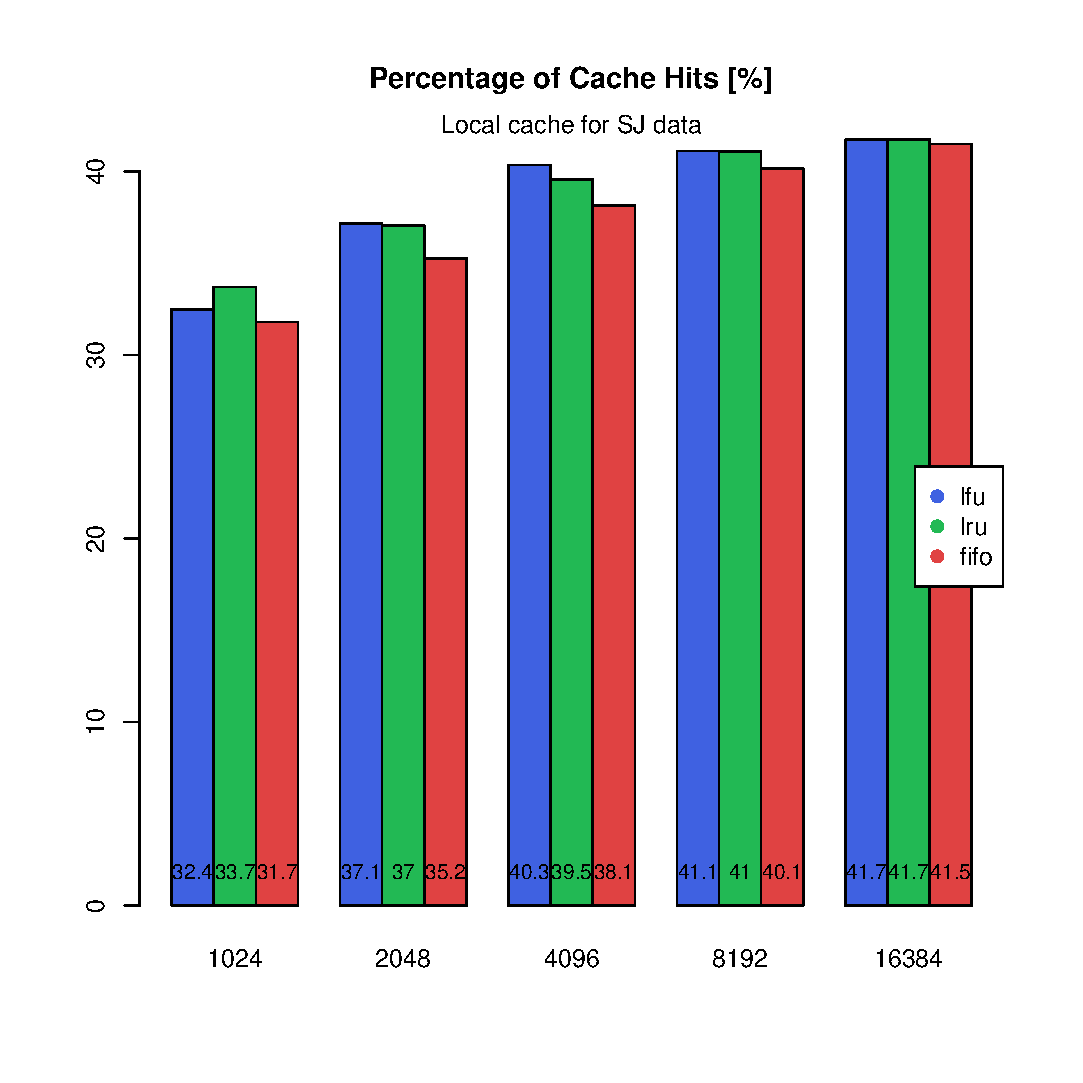
\includegraphics[width=0.9\linewidth]{img/tests/nop2p_sj_2.eps}
\end{minipage}
\begin{minipage}{0.48\linewidth}
\centering
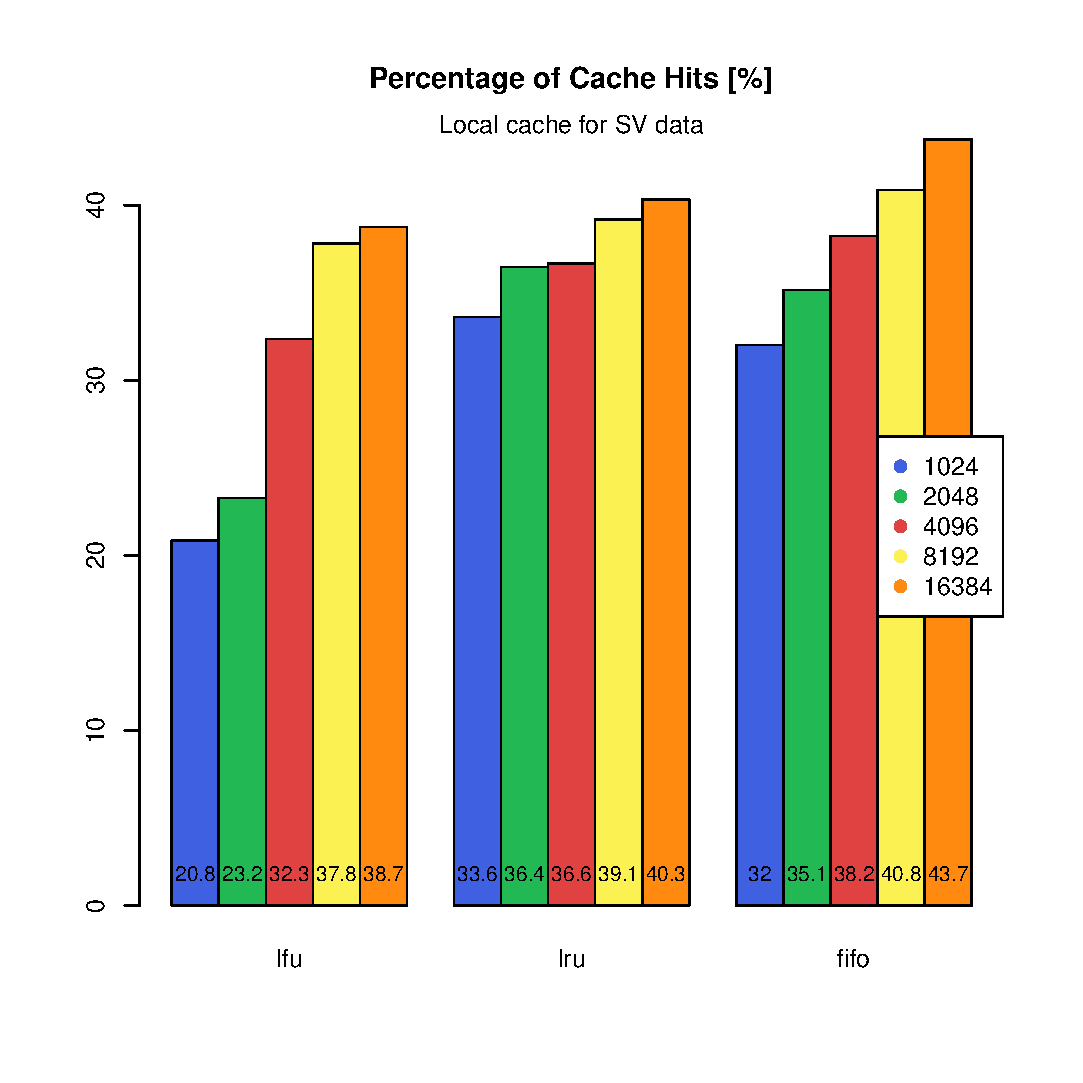
\includegraphics[width=0.9\linewidth]{img/tests/nop2p_sv_1.eps}
\end{minipage}
\begin{minipage}{0.48\linewidth}
\centering
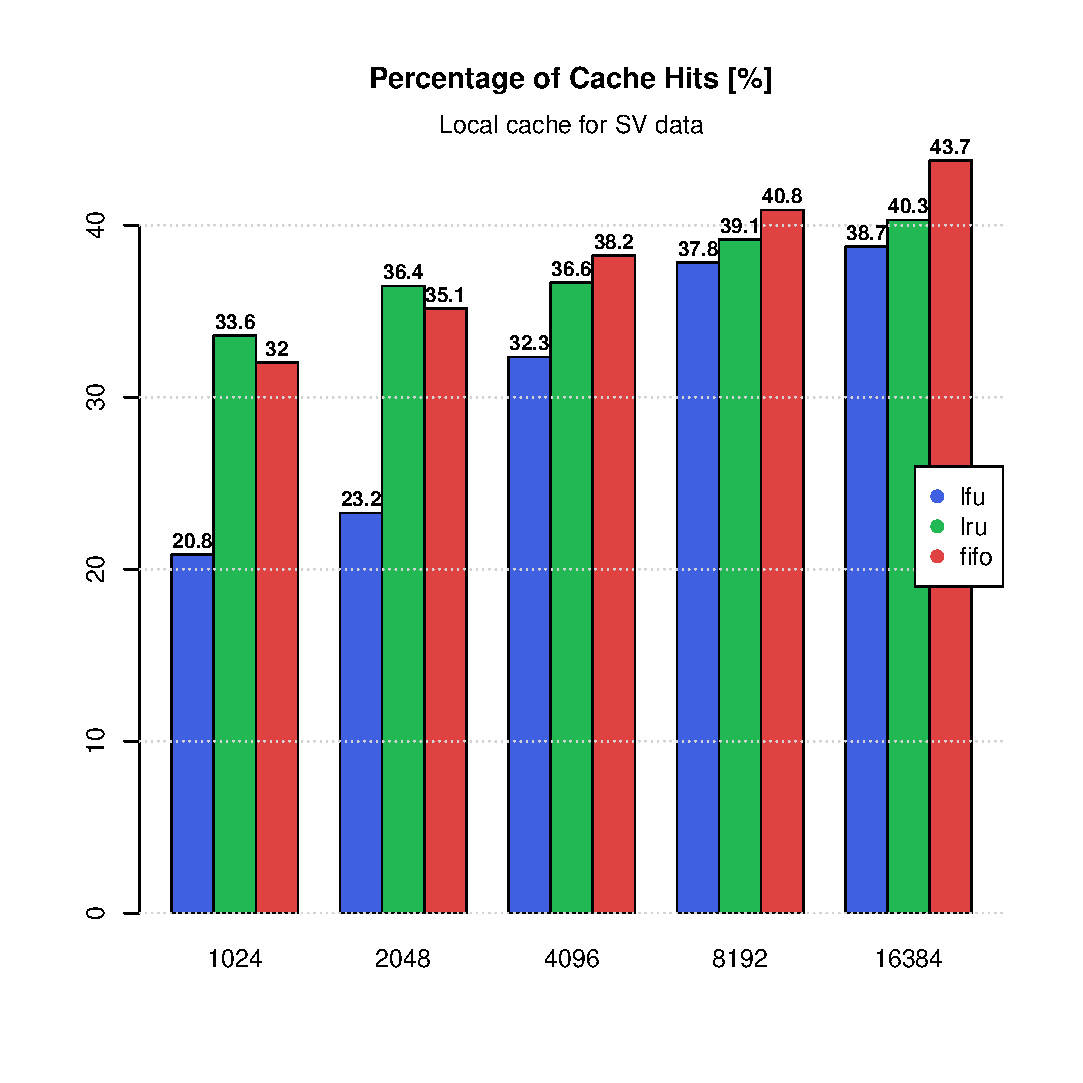
\includegraphics[width=0.9\linewidth]{img/tests/nop2p_sv_2.eps}
\end{minipage}
\begin{minipage}{0.48\linewidth}
\centering
\includegraphics[width=0.9\linewidth]{img/tests/nop2p_uc_1.eps}
\end{minipage}
\begin{minipage}{0.48\linewidth}
\centering
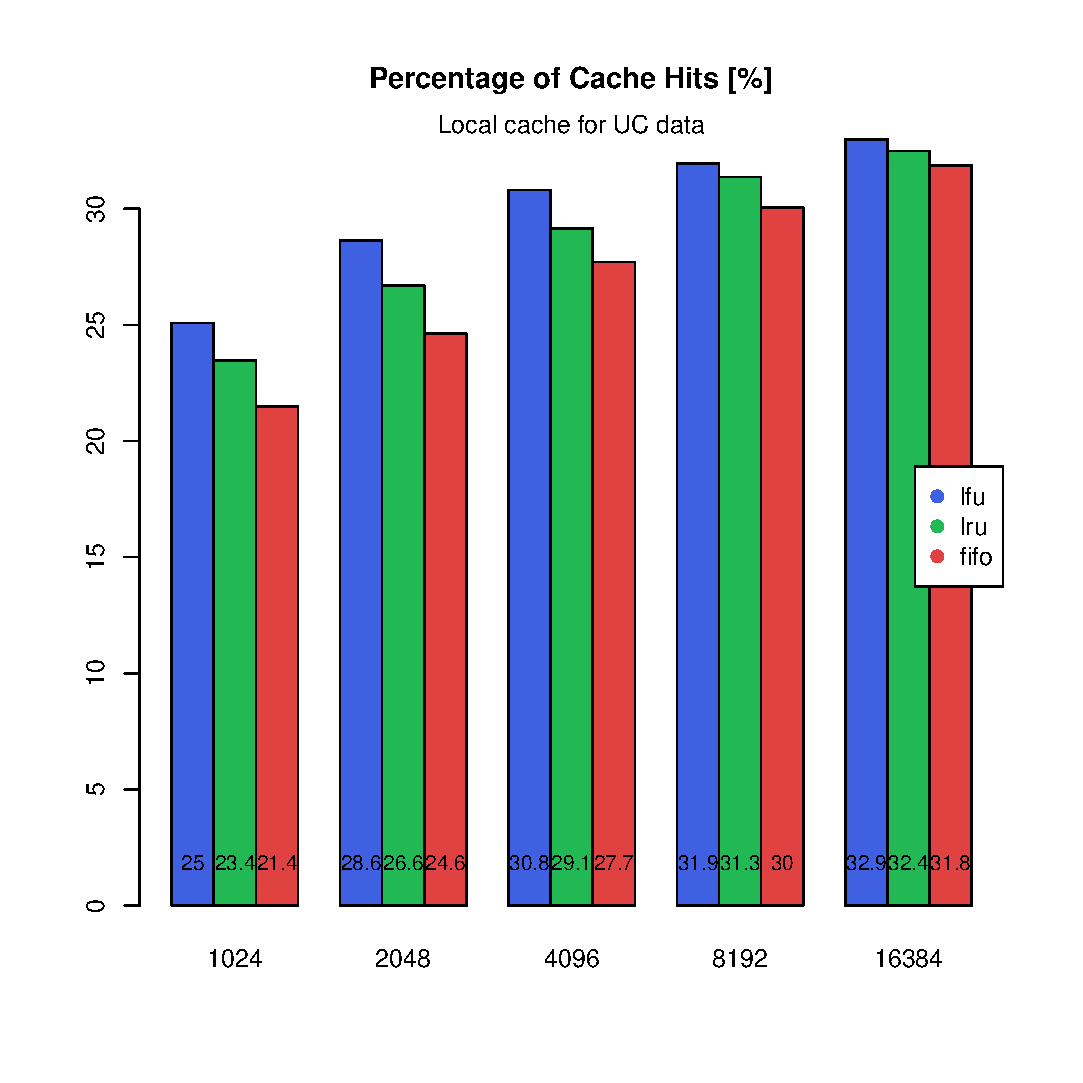
\includegraphics[width=0.9\linewidth]{img/tests/nop2p_uc_2.eps}
\end{minipage}
\caption{Wyniki testów \keszu\s lokalnego (w pamięci) dla przetestowanych zbiorów danych.}
\label{fig_tests_mem_all}
\end{figure}

\begin{figure}[h!]
\centering
\begin{minipage}{0.48\linewidth}
\centering
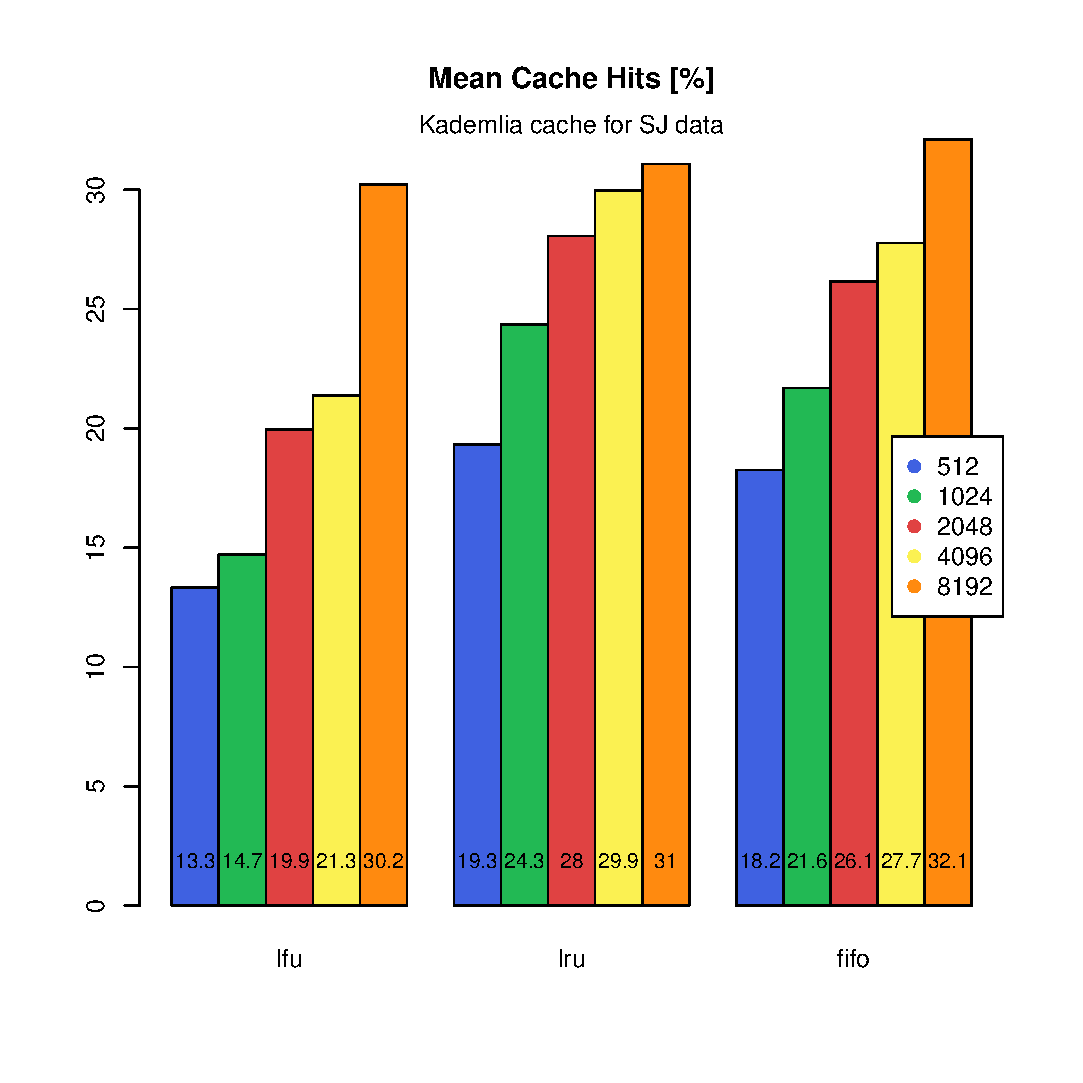
\includegraphics[width=0.9\linewidth]{img/tests/p2p_mean_sj_1.eps}
\end{minipage}
\begin{minipage}{0.48\linewidth}
\centering
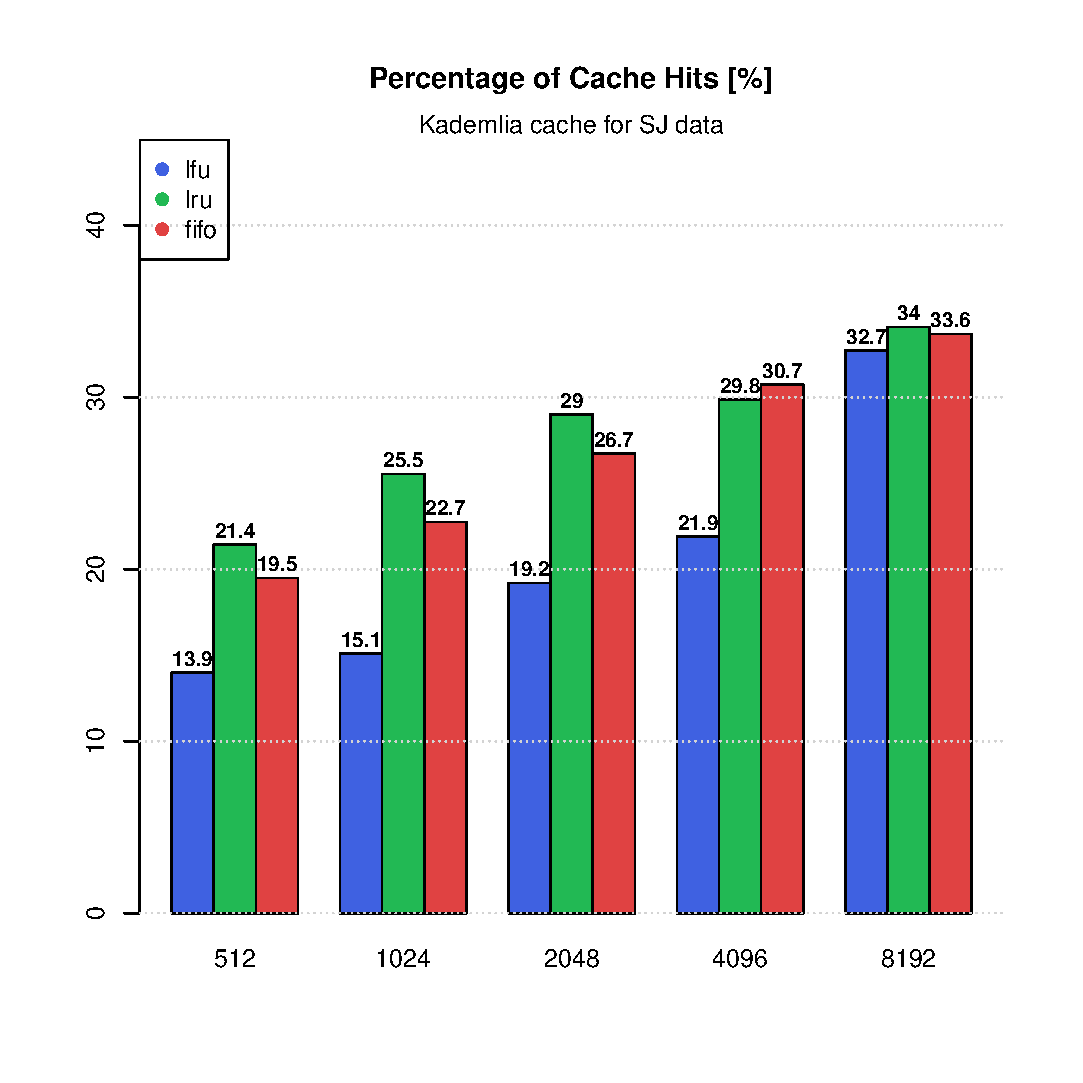
\includegraphics[width=0.9\linewidth]{img/tests/p2p_mean_sj_2.eps}
\end{minipage}
\begin{minipage}{0.48\linewidth}
\centering
\includegraphics[width=0.9\linewidth]{img/tests/p2p_mean_sv_1.eps}
\end{minipage}
\begin{minipage}{0.48\linewidth}
\centering
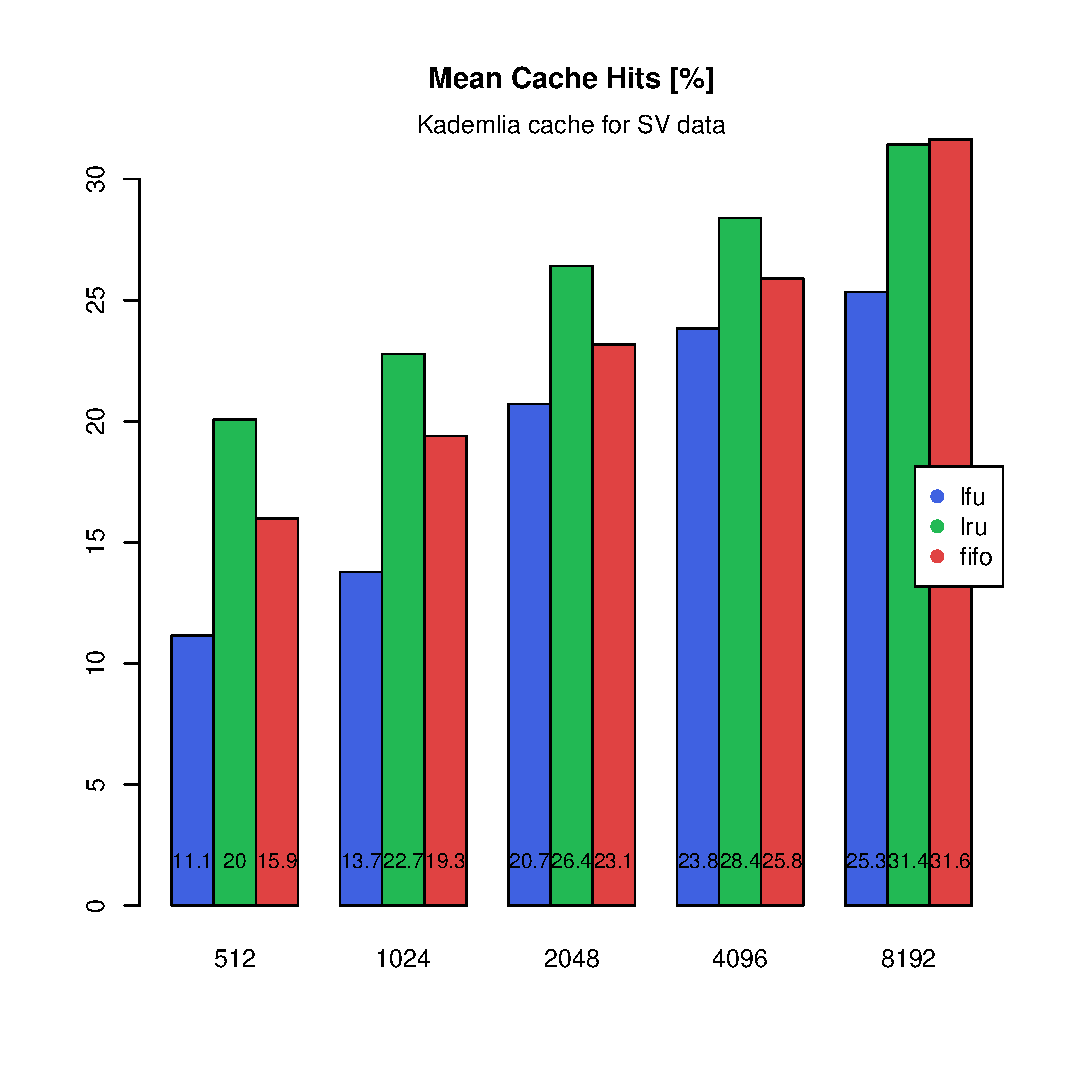
\includegraphics[width=0.9\linewidth]{img/tests/p2p_mean_sv_2.eps}
\end{minipage}
\begin{minipage}{0.48\linewidth}
\centering
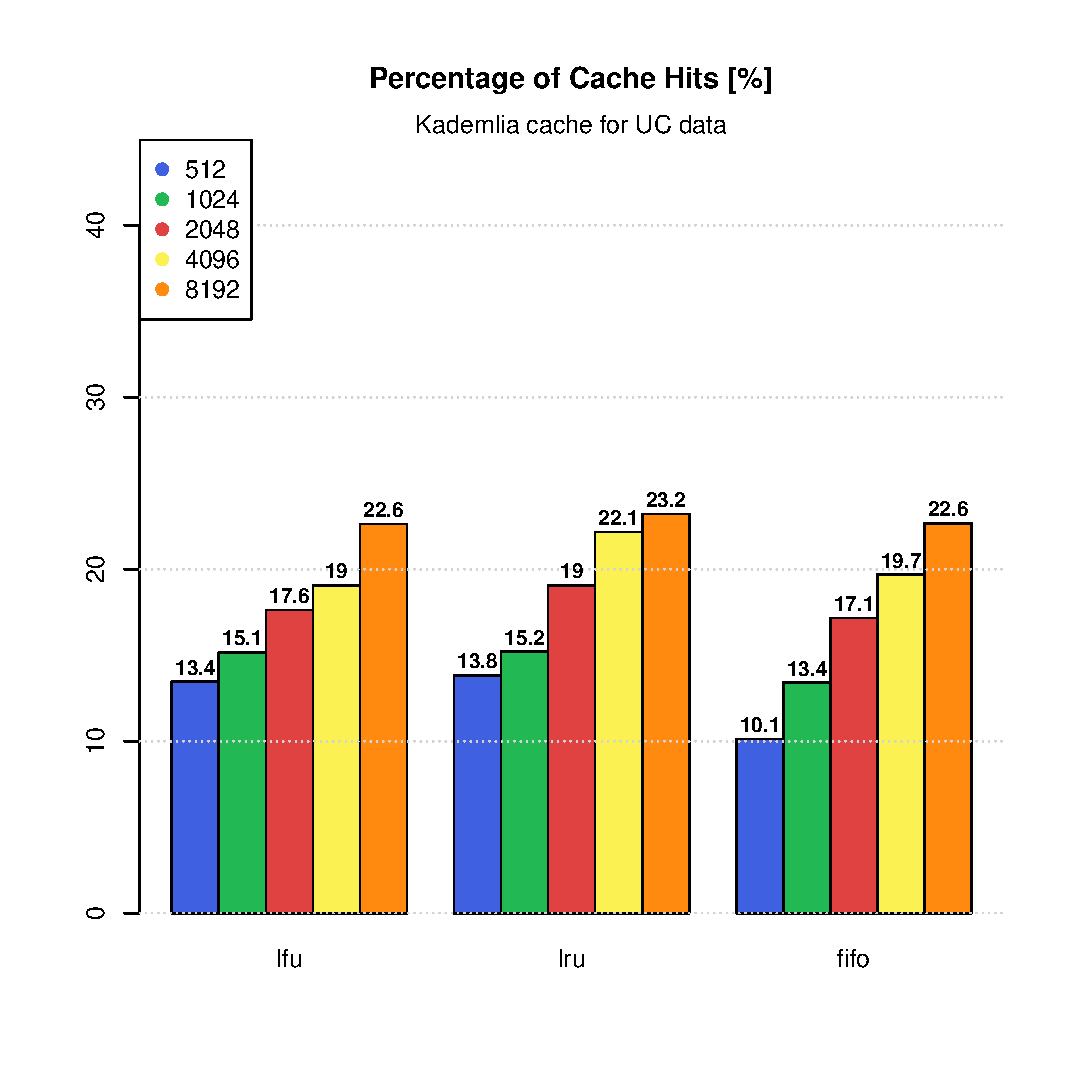
\includegraphics[width=0.9\linewidth]{img/tests/p2p_mean_uc_1.eps}
\end{minipage}
\begin{minipage}{0.48\linewidth}
\centering
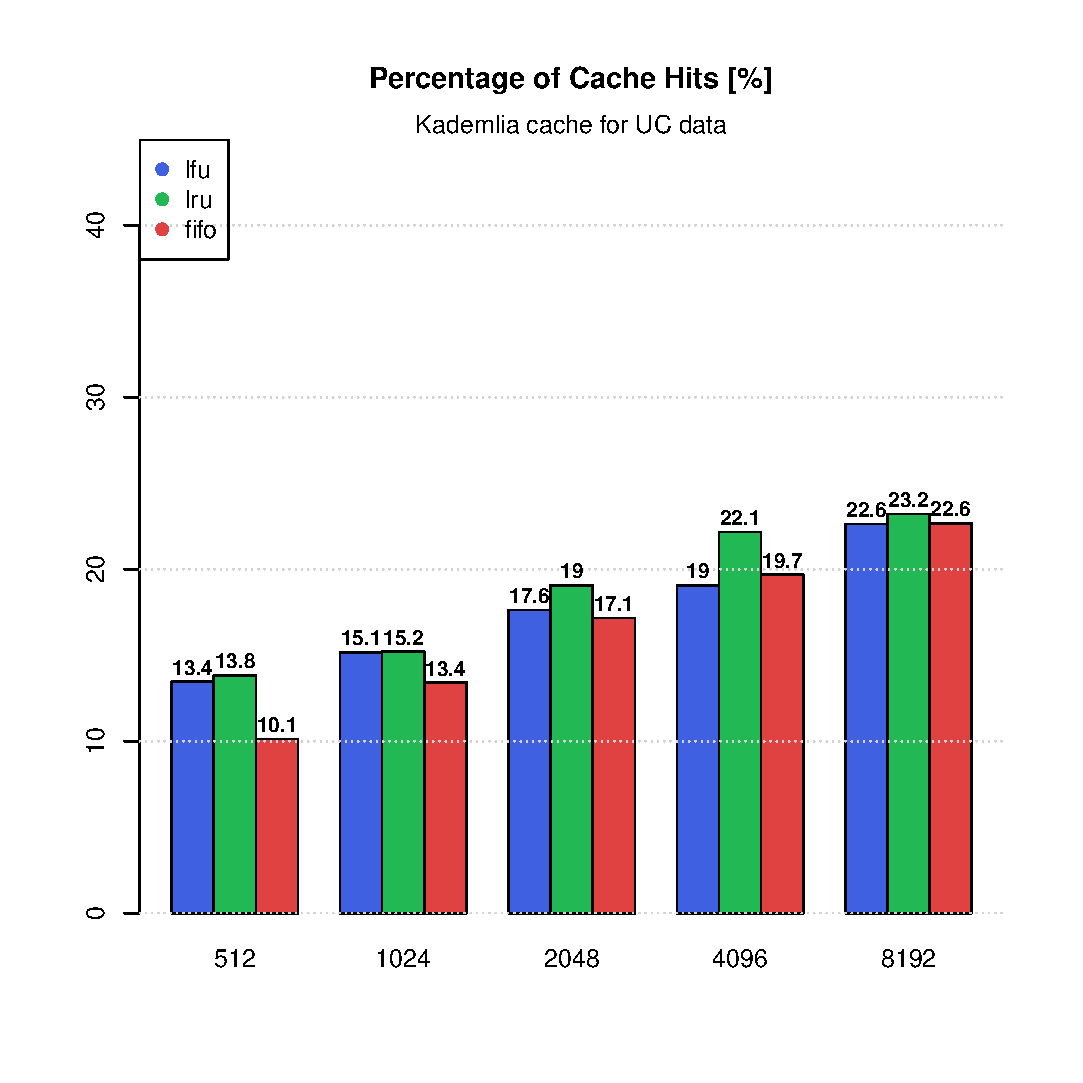
\includegraphics[width=0.9\linewidth]{img/tests/p2p_mean_uc_2.eps}
\end{minipage}
\caption{Uśrednione wyniki testów \keszu\s w sieci peer-to-peer dla przetestowanych zbiorów danych.}
\label{fig_tests_p2p_mean}
\end{figure}

\begin{figure}[h!]
\centering
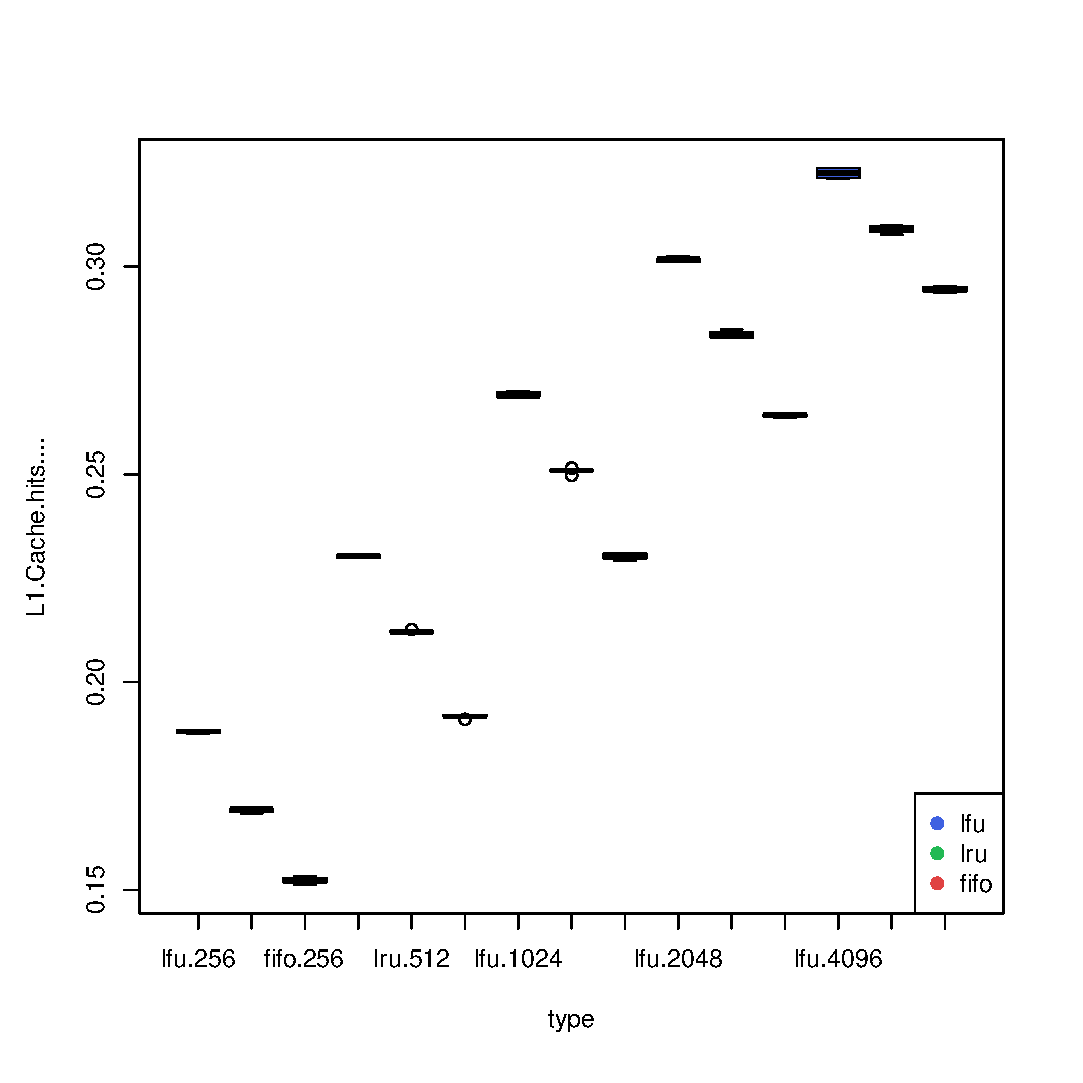
\includegraphics[width=0.6\linewidth]{img/tests/nop2p_all.eps}
\caption{Zbiorczy wykres wyników testów \keszu\s w pamięci dla wszystkich zbiorów danych.}
\label{fig_tests_mem_1}
\end{figure}

\begin{figure}[h!]
\centering
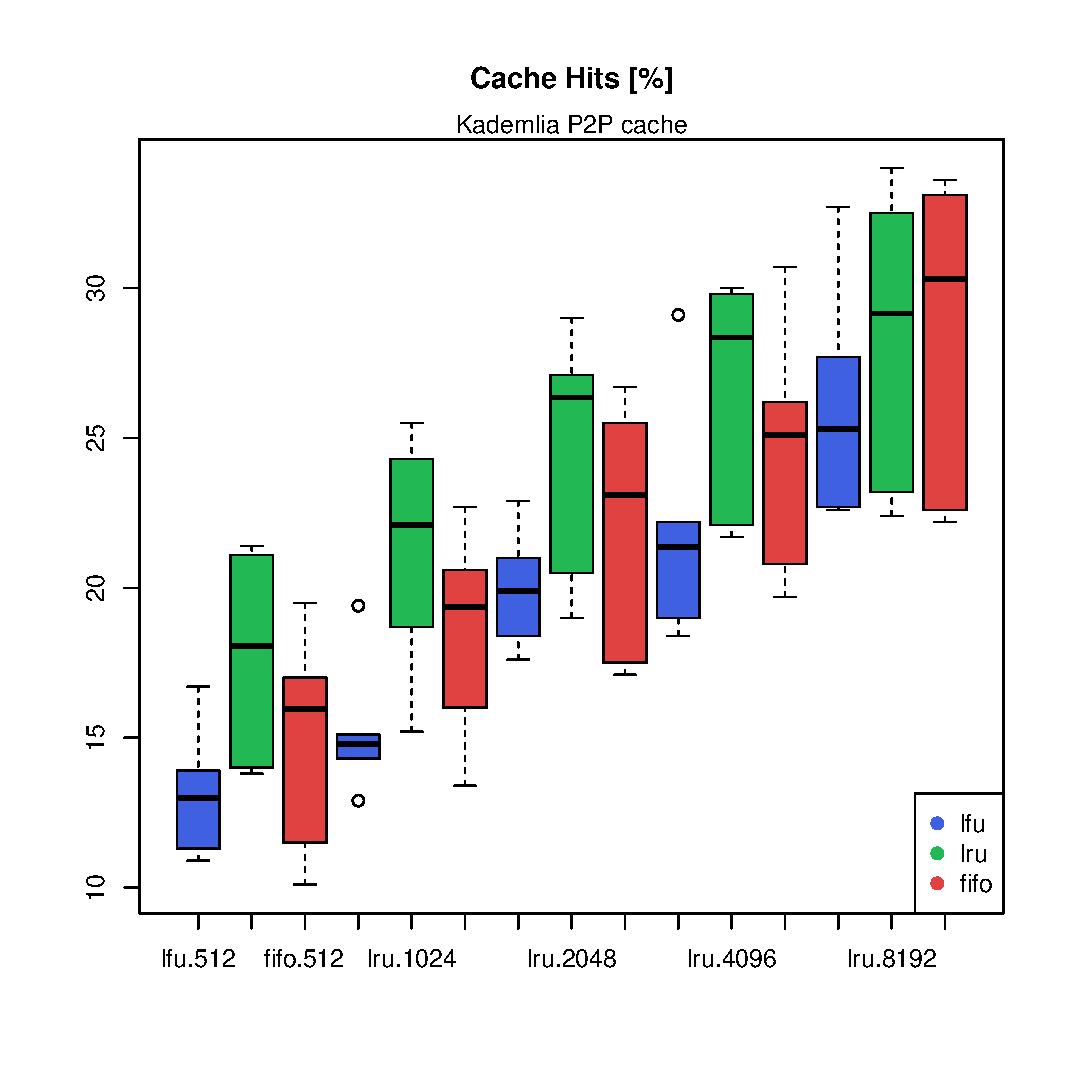
\includegraphics[width=0.6\linewidth]{img/tests/p2p_combined_all.eps}
\caption{Zbiorczy wykres wyników testów \keszu\s w sieci peer-to-peer dla wszystkich zbiorów danych.}
\label{fig_tests_p2p_all}
\end{figure}


\subsection{\Keszowanie\s w~sieci P2P}
Drugim przedmiotem testów było działanie \keszu, który wykorzystuje sieć peer-to-peer. Celem testów jest określenie w~jakim procencie dane, które pobierane są przez jednego użytkownika mogą zostać wykorzystane przez pozostałych.

Ponownie testy zostały przeprowadzadzone z~uwzględnieniem róznej wielkości \keszu\s oraz różnych algorytmów wymiany danych w~przypadku pełnego \keszu. Podczas testów wyłączony został zupełnie \kesz\s w~pamięci, aby zapytania o~wszystkie zasoby były wyszukiwane w~sieci peer-to-peer.

Ponieważ symulator, w~celu odwzorowania realnego środowiska pracy, tworzy procesy, które komunikują się ze sobą przez sieć, znacząco obciąża to komputer, na którym testy są uruchomione. Dodatkowo \textit{Kademlia} używa do komunikacji między węzłami protokołu \f{UDP}, który jest protokołem stratnym. z~powyższych powodów nie wszystkie wysłane zapytania są poprawnie obsłużone - część z~wysyłanych pakietów nie dociera do celu, co skutkuje przekroczeniem limitów czasów zdefiniowanych w~protokole \textit{Kademli} i~pomimo, że zasób może znajdować się w~sieci istnieje szansa, że w~czasie testów wyszukiwanie zasobu zakończy się niepowodzeniem.
Dla przedstawionych wyników testów średnio $91\%$ zapytań została obsłużona poprawnie. Pozostałe zakończyły się niepowodzeniem z powodu utraty pakietu \f{UDP} lub z powodu upłynięcia limitu czasu przewidzianego na odpowiedź ustalonego na 5 sekund.

Podobnie jak w~przypadku testów w~pamięci (rozdział~\ref{sect_tests_mem}) przetestowane zostały trzy algorytmy \keszowania\s, ale o~wielkościach 512, 1024, 2048, 4096 i~8192.

Na rysunku \ref{fig_tests_p2p_mean} przedstawione zostały średnie wartości procentu zasobów, które były \keszowane dla poszczególnych zbiorów danych. Wyniki pochodzą z kilku niezależnych uruchomień symulatora na różnych maszynach. Rysunek \ref{fig_tests_p2p_all} przedstawia zebrane wyniki dla wszystkich zbiorów danych.

\subsection{\Keszowanie\s dwupoziomowe}
Ostatnie z~przeprowadzonych testów dotyczą połączenia lokalnego \keszowania\s w~pamięci z~\keszowaniem\s w~sieci peer-to-peer. W~tym celu wykorzystywane jest \keszowanie\s dwupoziomowe - w~pierwszej kolejności sprawdzany jest \kesz\s lokalny, a~dopiero w~przypadku, gdy zasób nie zostaniem znaleziony w~pamięci, zapytanie wysyłane jest do sieci peer-to-peer.

Do testów użyte zostały następujące parametry

TODO: odpalenie symulacji nieprzyspieszonej (albo przyspieszonej mniej)
TODO: Dobranie odpowiednich algorytmów i~wielkości kolejek
TODO: porównanie opóźnień na chordzie i kademli.

\begin{figure}[h!]

\caption{Porównanie średniego opóźnienia pomiędzy Kademlią i Chordem.}
\label{fig_latency}
\end{figure}

\subsection{Wnioski}
TODO: Wnioski wynikające z~testów

Wyniki testów dla \keszu\s lokalnego znacząco różnią się w zależności od zbioru danych. Oczywiście w przypadku wszystkich algorytmów \keszowania\s zwiększanie rozmiaru \keszu\s powoduje wzrost liczby trafień (ang. \textit{Cache hit}). Dla wszystkich danych można zaobserwować ciekawą zależność: dla wielkości powyżej 2048 liczby trafień dla wszystkich polityk \keszowania\s się wyrównują. Związane jest to z tym, że dla większości klientów liczba zapytań jest większa od $2^{11}$ i mniejsza od $2^{12}$.

Dla danych \f{UC} najlepsze wyniki daje \kesz\s LFU. Podobnie jest dla zbioru \f{SJ}, chociaż tam wyniki poszczególnych algorytmów są bardziej wyrównane. W przypadku \f{SV} do wspomnianej już wartości granicznej 2048 najlepiej radzi sobie poityka LRU, a dla pozostałych wartości lepsze wyniki daje zastosowanie FIFO. Wyniki są o tyle ciekawe, że LRU i FIFO działają bardzo podobnie, LRU pozwala jedynie na uaktualnienie pozycji w przypadku odwołania do elementu, który znajduje się już w \keszu. Jednak w specyficznym przypadku danych \f{SV} własność ta obniża liczbę trafień.
Wartości liczby trafień są podobne dla zbiorów \f{SJ} i \f{SV}, LRU pozwala na uzyskanie od $33\%$ dla \keszu\s wielkości 1024 do $41\%$ trafień dla \keszu\s wielkości 16384. Dla zbioru \f{UC} wyniki wynoszą odpowiednio $23\%$ i $32\%$.

Uśrednione wyniki dla wszystkich zbiorów danych przedstawione na rysunku \ref{fig_tests_mem_1} pokazują, że w średnim przypadku najlepiej zachowuje się polityka LRU. Wynik ten potwierdza poprzednio uzyskane wyniki \cite{breslau1999web} i uzasadnia popularność tego algorytmu w systemach \keszowania. 

W przypadku \keszowania\s w sieci peer-to-peer ponownie zwiększenie rozmiaru \keszu\s bezpośrednio wpływa na liczbę trafień. Również tutaj najlepsze wyniki oferowane są przez politykę LRU. Główną różnicą w wynikach dla sieci peer-to-peer są wartośći dla liczby trafień. Wyniki dla LRU dla zbiorów \f{SV} i \f{SJ} wynoszą około $20\%$ w przypadku \keszu\s o wielkości 512 do $30\%$ dla wielkości $8192$. Dla zbioru \f{UC} wyniki podobnie jak w przypadku \keszowania\s w pamięci są nieco gorsze od pozostałych zbiorów i kształtują się na poziomie od $14\%$ do $23\%$.


TODO: coś o testach kompleksowych

Na wykresie \ref{fig_latency} możemy zaobserwować ogromną dyspropocję pomiędzy średnim opóźnieniem na obsługę zapytania w przypadku Kademlii i Chorda. Jedną z przyczyn takiej różnicy jest brak równoległych zapytań w przypadku Chorda - jeżeli węzeł, którego chcemy odpytać nie jest już dostępny to protokół musi poczekać na ustalony limit czasowy i dopiero wtedy rozpocząć odpytywanie innego węzła. Drugi powodem jest słaba jakość biblioteki użytej do obsługi Chorda\footnote{\f{http://code.google.com/p/pyrope/}}, wszystkie procedury są tam zaimplementowane w sposób blokujący, więc w przypadku gdy wiele węzłów opuści sieć zapytania blokowane są przez oczekiwanie na odpowiedź z poprzednio wysłanych żądań.


\section{Implementacja}
\label{sect_impl}
W niniejszym rozdziale opisujemy implementację rozproszonego \keszu\s z~użyciem DHT. W~rozdziale~\ref{sect_impl_technology}
przedstawimy podjęte próby innej formy implementacji, a~w rozdziale~\ref{sect_impl_proxy} opiszemy ostatecznie wybrane rozwiązanie.
Rozdział~\ref{sect_impl_install} prezentuje informacje o~instalacji i~uruchomieniu stworzonego programu.

\subsection{Wybór technologii}
\label{sect_impl_technology}
Wybór technologii był silnie zależny od celu, który chcieliśmy osiągnąć. Początkowo istotnym aspektem, był aspekt praktyczny tworzonego rozwiązania, priorytetem było maksymalne uproszczenie i~ułatwienie procesu instalacji \keszu, tak aby jak najwięcej osób było chętnych przetestować system. Celem było zebranie danych do testów oraz analiza działania i~uzyskiwanych opóźnień podczas normalnej pracy programu. z~tego powodu przed implementacją ostatecznego rozwiązania opisanego w~rozdziale~\ref{sect_impl_proxy} podjęte zostały próby utworzenia pluginu do przeglądarki, opisane w~rozdziałach~\ref{sect_plugin_1} i~\ref{sect_plugin_2}.

\subsubsection{Plugin do przeglądarki}
\label{sect_plugin_1}
Pierwszą podjętą próbą implementacji było stworzenie rozszerzenia do przeglądarki Chrome\footnote{\url{http://chrome.google.com}}, które korzystałoby z~nowego API dla połączeń Peer-to-peer, zaproponowanego w~HTML5\footnote{\url{http://www.w3.org/TR/2008/WD-html5-20080122/#peer-to-peer}, \url{http://www.w3.org/TR/webrtc}}.

Jako \textit{proof-of-concept} stworzony został plugin, którego kod znajduje się na listingu~\ref{lst_plugin_1}.

\begin{lstlisting}[language={JavaScript}, label={lst_plugin_1}, 
  caption={Kod rozszerzenia dla przeglądarki Chrome, realizujący \textit{proof-of-concept}.}]
(function() { 'use strict';
var cowImg;
chrome.webRequest.onBeforeRequest.addListener(function(details){
  // Don't redirect multiple times
	if (loldogs.indexOf(details.url) !== -1) {
		return;
	}
	
  // Redirect to cow
	var url = cowImg;
  // or to loldogs
	if (Math.random() < .5) {
		url = loldogs[Math.round(Math.random() * loldogs.length)];
	}
	
	console.log("Redirecting", details.url, " to ", 
    (url === cowImg ? "COW" : url));
    
  // Return redirection url
	return {
		redirectUrl: url
	};
}, {
	urls: ['<all\_urls>'],
	types: ['image']
}, ["blocking"]);

cowImg = "data:image/png;base64,iVBORw0KG...";
}());
\end{lstlisting}

Rozwiązanie korzysta z~API \f{chrome.webRequest.onBeforeRequest}\footnote{\url{http://developer.chrome.com/extensions/webRequest.html}}, które pozwala nasłuchiwać oraz modyfikować wszystkie żądania, wychodzące z~przeglądarki. Nasłuchiwane są tylko żądania o~obrazki, z~dowolnymi adresami URL. Następnie każde żądanie z~prawdopodobieństwem $\nicefrac{1}{2}$ zostaje zastąpione obrazkiem \f{cowImg}, który znajduje się w~pliku źródłowym w~zakodowanej postaci (\f{base64}) oraz z~prawdopodobieństwem $\nicefrac{1}{2}$ jednym z~obrazków z~tablicy \f{loldogs}. Dzięki przekierowaniu na zasób w~postaci \f{base64} nie jest konieczne wykonywanie dodatkowego żądania przez przeglądarkę i~obrazek jest wyświetlany od razu. 

Niestety stworzenie tego pluginu pokazało poważną wadę tego podejścia. Żeby przechwytywać żądania w~trybie \f{onBeforeRequest}, czyli przed wykonaniem zapytania przez przeglądarkę musimy korzystać z~opcji \f{blocking}, która powoduje, że żądania muszą być przetwarzane synchronicznie. Zatem próby pobrania zasobu z~sieci P2P podczas przechwytywania zapytania będą skutkowały zwiększonymi opóźnieniami w~dostępie do zasobów, co podważa podstawową ideę rozwiązania.

\subsubsection{Plugin \textit{Native Client}}
\label{sect_plugin_2}
Kolejnym podejściem było stworzenie pluginu dla przeglądarki Chrome w~technologii \textit{Native Client (NaCL)}. \textit{NaCL} pozwala na kompilację programów, które uruchamiane są w~piaskownicy (ang. \textit{sandboxed environment}) w~celu zapewnienia bezpieczeństwa użytkownika. Główną zaletą technologii jest wydajność, która jest bliska wydajności natywnych aplikacji.

Pomimo ogłoszenia przez Google gotowości \textit{Native Client} do produkcyjnego użycia, plugin nie został stworzony z~powodu słabej dokumentacji oraz braku wersji odpowiednich bibliotek na platformie \textit{NaCL}.

\subsection{Proxy \keszujace}
\label{sect_impl_proxy}
Po nieudanych próbach stworzenia rozszerzenia do przeglądarki stworzone zostało rozwiązanie, które wymaga dodatkowej instalacji i~konfiguracji systemu, ale bazuje na znanych i~dobrze przetestowanych komponentach. Ostateczną aplikacją jest proxy \keszujace, w~którym każde zapytanie (wykluczając ruch \f{https}) jest przekazywane do oryginalnego serwera tylko w~momencie, gdy nie zostanie znalezione w~\keszu.

Program został wykonany w~języku \f{Python} z~użyciem bibliotek \f{Twisted}\footnote{\url{http://twistedmatrix.com}} oraz \f{Entangled}\footnote{\url{http://entangled.sourceforge.net}}. Aplikacja składa się z~dwóch części:
\begin{description}
  \item[Proxy]{ - serwer proxy, który odpowiada za przekazywanie zapytań oraz odpytywanie \keszu\s o~zasoby,}
  \item[P2P]{ - klient sieci Peer-to-Peer, pozwalający na odszukiwanie zasobów, które w~tej sieci się znajdują.}
\end{description}
Na rysunku~\ref{fig_architecture} w~rozdziale~\ref{sect_architecture} przedstawione zostało przykładowe zapytanie i~jego droga przez poszczególne komponenty aplikacji. 

\subsection{Symulator}
\label{sect_impl_simulator}
W celu wykonania testów, których wyniki przedstawione zostały w~rozdziale~\ref{sect_tests} wykonany został symulator bazujący na stworzonej aplikacji. 

Symulator pozwala na wczytanie danych o~klientach i~żądaniach, które mają wykonać. Każdy z~klientów jest osobnym procesem, który uruchamiany jest przez proces główny symulatora (skrypt \f{simulator\_main.py}). Wyniki symulacji zapisywane są do pliku z~logami i~zawierają identyfikator \keszu, z~którego otrzymano zasób (lub $-1$ w~przypadku, gdy zasób nie został znaleziony w~żadnych \keszu) oraz opóźnienie, czyli czas, który upłynął od wysłania zapytania do otrzymania odpowiedzi.

\subsection{Skrypty pomocnicze}
Aby ułatwić przetwarzania plików z~logami zostały wykonane pomocnicze skrypty dla środowiska \f{R}\footnote{\url{http://www.r-project.org}}. 

Pierwszy ze skryptów (\f{read.data.r}) odpowiedzialny jest za wczytanie danych testowych i~przetworzenie ich na format, które oczekuje symulator. Skrypt wczytuje więc plik z~logami z~serwera, który zawiera wpisy dla wszystkich żądań i~dzieli go na pliki z~zapytaniami dla poszczególnych klientów. Dodatkowo czas zapytań zamieniany jest z~bezwzględnego na relatywny, czyli pierwsze zapytanie ma czas $0$, a~czas pozostałych to opóźnienie w~stosunku do pierwszego żądania.

Skrypt \f{read.logs.r} pozwala na wczytanie danych wyjściowych z~symulatora i~opracowanie na ich podstawie wykresów odpowiedzi z~poszczególnych \keszy. Skrypt zapisuje też uproszczone wyniki symulacji, które używane są przez ostatni ze skryptów (\f{combine.logs.r}). Ponieważ wyniki symulacji są w~pewnym stopniu losowe (co wynika z~użycia protokołu UDP dla sieci \textit{Kademlia} oraz różnego obciążenia maszyny, na której uruchomione były symulacje) ostatni skrypt zbiera wyniki z~wielu uruchomień symulatora i~prezentuje wykresy z~uśrednionymi wynikami.

\subsection{Instalacja i~uruchomienie}
\label{sect_impl_install}
Aplikacja, jej źródła oraz niniejsza praca dostępne są na dołączonej płycie CD oraz publicznym repozytorium\footnote{\url{https://bitbucket.org/tomusdrw/mgr.p2p.proxy}}. W~celu uruchomienia aplikacji wymagany jest \f{Python} w~wersji \f{2.7} oraz pakiety \f{python2.7-twisted} i~\f{python2.7-simplejson}. Aby pobrać źródła aplikacji można skorzystać z~polecenia \f{\$ git clone git@bitbucket.org:tomusdrw/mgr.p2p.proxy.git}.

Uruchomienie aplikacji odbywa się przez wywołanie pliku \f{main.py}, znajdującego się w~głównym katalogu. Rysunek~\ref{fig_main_help} przedstawia dostępne opcje konfiguracyjne.

\begin{figure}[h]
\centering
\includegraphics[width=0.8\linewidth]{img/options.png}
\caption{Dostępne opcje konfiguracyjne głównej aplikacji.}
\label{fig_main_help}
\end{figure}

Wywołanie symulatora możliwe jest przez uruchomienie programu \f{simulator\_main.py}. Symulator przyjmuje podobne opcje co główna aplikacja. Dodatkowo do pracy symulatora potrzebne są dane wejściowe, które powinny znajdować się w~katalogu \f{simulator/data/}. Przykładowe dane zostały załączone w~repozytorium.

Dodatkowo w~celu uruchomienia wielu symulacji utworzone zostały pomocnicze skrypty dla konsoli \f{bash}: \f{run\_nomem\_simulations.sh} oraz \f{run\_nop2p\_simulations.sh}. Pozwalają one na uruchomienie symulacji odpowiednio \keszu\s lokalnego i \keszu\s w sieci peer-to-peer dla różnych algorytmów \keszowania\s i~wielkości \keszy.


\section{Podsumowanie}

Przygotowany w ramach pracy system oferuje
TODO: Podsumowanie tego co zostało zrobione, interpretacja wyników i~ogólnie trochę wody.

\bibliographystyle{plain}

\bibliography{document}

\end{document}
